% UNIVERSAL SETTINGS
% document structure
\documentclass[12pt,twoside,onecolumn,openright,extrafontsizes]{memoir}
\usepackage[utf8x]{inputenc}

% ebgaramond font package
\usepackage[cmintegrals,cmbraces]{newtxmath}
\usepackage{ebgaramond-maths}
\usepackage[T1]{fontenc}

% Predefined commands
\newcommand*\NewPage{\newpage\thispagestyle{empty}\mbox{}}

% Text macros
\def\chichenitza*{Chich\'{e}n Itz\'{a}}

% PACKAGE DEFINITION
% typographical packages
\usepackage{microtype} % for micro-typographical adjustments
\usepackage{setspace} % for line spacing
\usepackage{lettrine} % for drop caps and awesome chapter beginnings
	\renewcommand{\LettrineTextFont}{\normalfont}
\usepackage{titlesec} % for manipulation of chapter titles

% for placeholder text
\usepackage{lipsum} % to generate Lorem Ipsum

% graphics package
\usepackage{wrapfig}
\usepackage{graphicx}
\graphicspath{Images/}
\newcommand{\parasep}{
	\begin{center} 
		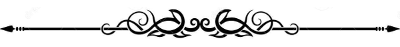
\includegraphics[scale=.5]{Images/hrule.png} 
	\end{center}}


% other
\usepackage{calc}
\usepackage{hologo}
\usepackage[hidelinks]{hyperref}
\usepackage{verbatim}


% PHYSICAL DOCUMENT SETUP
% media settings
\setstocksize{8.5in}{5.675in}
\settrimmedsize{8.5in}{5.5in}{*}
\setbinding{0.175in}
\setlrmarginsandblock{0.611in}{1.222in}{*}
\setulmarginsandblock{0.722in}{1.545in}{*}
\setlength{\parindent}{0.5em}

% defining the title and the author
\title{Susan Rodriguez: The Quickening}
\author{Eric B. Teepell}
\newcommand{\press}{Susan's Requiem series prequel}

% custom second title page
\makeatletter
\newcommand*\halftitlepage{\begingroup % Misericords, T&H p 153
  \setlength\drop{0.1\textheight}
  \begin{center}
  \vspace*{\drop}
  \rule{\textwidth}{0in}\par
  {\Large\textsc\thetitle\par}
  \rule{\textwidth}{0in}\par
  \vfill
  \end{center}
\endgroup}
\makeatother

% custom title page
\thispagestyle{empty}
\makeatletter
\newlength\drop
\newcommand*\titleM{\begingroup % Misericords, T&H p 153
  \setlength\drop{0.15\textheight}
  \begin{center}
  \vspace*{\drop}
  \rule{\textwidth}{0in}\par
  {\HUGE\textsc\thetitle\par}
  \rule{\textwidth}{0in}\par
  {\Large\textit\theauthor\par}
  \vfill
  {\Large\scshape\press}
  \end{center}
\endgroup}
\makeatother

% chapter title manipulation
% padding with zero
\renewcommand*\thechapter{\ifnum\value{chapter}<10 0\fi\arabic{chapter}}
% chapter title display
\titleformat
{\chapter}
[display]
{\normalfont\scshape\huge}
{\HUGE\thechapter\centering}
{0pt}
{\vspace{18pt}\centering}[\vspace{42pt}]

% typographical settings for the body text
\setlength{\parskip}{0em}
\linespread{1.04}

% HEADER AND FOOTER MANIPULATION
  % for normal pages
  \nouppercaseheads
  \headsep = 0.16in
  \makepagestyle{mystyle} 
  \setlength{\headwidth}{\dimexpr\textwidth+\marginparsep+\marginparwidth\relax}
  \makerunningwidth{mystyle}{\headwidth}
  \makeevenhead{mystyle}{}{\textsf{\scriptsize\scshape\thetitle}}{}
  \makeoddhead{mystyle}{}{\textsf{\scriptsize\scshape\leftmark}}{}
  \makeevenfoot{mystyle}{}{\textsf{\scriptsize\thepage}}{}
  \makeoddfoot{mystyle}{}{\textsf{\scriptsize\thepage}}{}
  \makeatletter
  \makepsmarks{mystyle}{%
  \createmark{chapter}{left}{nonumber}{\@chapapp\ }{.\ }}
  \makeatother
  % for pages where chapters begin
  \makepagestyle{plain}
  \makerunningwidth{plain}{\headwidth}
  \makeevenfoot{plain}{}{}{}
  \makeoddfoot{plain}{}{}{}
  \pagestyle{mystyle}
% END HEADER AND FOOTER MANIPULATION

% table of contents customisation
\renewcommand\contentsname{\normalfont\scshape Contents}
\renewcommand\cftchapterfont{\normalfont}
\renewcommand{\cftchapterpagefont}{\normalfont}
\renewcommand{\printtoctitle}{\centering\Huge}

% layout check and fix
\checkandfixthelayout
\fixpdflayout

% BEGIN THE DOCUMENT
\begin{document}
\pagestyle{empty}
% the half title page
\halftitlepage
\cleardoublepage
% the title page
\titleM
\clearpage
% copyright page
\noindent{\small{This novel is entirely a work of fiction. The names, characters and incidents portrayed in it are the product of the author's imagination. Any resemblance to actual persons, living or dead, or events or localities is entirely coincidental.\par\vfill\noindent Pre-Draft Edition\space\today\\
		% ISBN\space\ISBN\\
		Source: https://eteepell.github.io/Susans-Requiem/\\
		\copyright\space\theauthor.   \par\vfill\noindent\theauthor\space asserts the moral right to be identified as the author of this work. This work is licensed under a Creative Commons Attribution-ShareAlike 4.0 International License.\par }}

\begin{center}
 	\centering
	
\includegraphics[width=0.25\linewidth=0.25]{license}
\end{center}

\newpage
{\tiny Disclaimer This deed highlights only some of the key features and terms of the actual license. It is not a license and has no legal value. You should carefully review all of the terms and conditions of the actual license before using the licensed material. You are free to: Share — copy and redistribute the material in any medium or format Adapt — remix, transform, and build upon the material
for any purpose, even commercially. The licensor cannot revoke these freedoms as long as you follow the license terms. Under the following terms: Attribution — You must give appropriate credit, provide a link to the license, and indicate if changes were made. You may do so in any reasonable manner, but not in any way that suggests the licensor endorses you or your use. ShareAlike — If you remix, transform, or build upon the material, you must distribute your contributions under the same license as the original. No additional restrictions — You may not apply legal terms or technological measures that legally restrict others from doing anything the license permits. Notices: You do not have to comply with the license for elements of the material in the public domain or where your use is permitted by an applicable exception or limitation. No warranties are given. The license may not give you all of the permissions necessary for your intended use. For example, other rights such as publicity, privacy, or moral rights may limit how you use the material.
}
\clearpage

% dedication
\begin{center}
\itshape{\noindent{Dedicated to queen Lilith, Dresden Files Readers, and \LaTeX \: users worldwide.}}
\end{center}

% begin front matter
\frontmatter
\pagestyle{mystyle}
%
%\chapter*{Dedication to Queen Lilith}
%{Bear with me here, \textit{Queen Lilith is the actual god and queen of vampires}. The real one, insofar as there could be.
%	
%I've done some research as I went along, what writer doesn't. I was creatively inspired to write about what happened to Susan on the alter of \chichenitza*. How she stood against the odds and will change the world for the better. The story of a hero who just happens to be a vampire physically. Somebody decent, with a dangerous side. I started it two or three months ago.
%
%I've avoided looking too much into vampire lore. The reason being I believed it would be horrible, mean and nasty. Either in the horror sense or in the campy sense.
%
%That isn't what I wanted to show in Susan. Neither maniacal nor glittery. I wanted to break the mold of vampire novels and \textit{not write a vampire novel.} I would write about an antihero trying to make a positive difference in the world without brooding a lot. That's gotten very annoying with other protagonists over the years. 
%
%I wanted to show strength, confidence, determination, responsibility, and someone protective and nurturing. A female hero that stands alone. A female hero that can be truly intimidating, and lay down some serious kick ass when it needs to be done. 
%
%\begin{wrapfigure}{R}{0.5\textwidth}
%	\centering
%	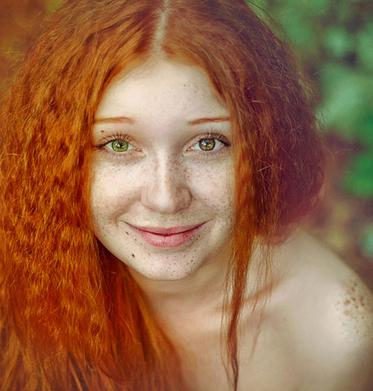
\includegraphics[width=0.50\textwidth]{Images/ginger-girl}
%	\\ {\small Lilith, Queen of Night and Darkness.}
%\end{wrapfigure}
%
%About a month ago or a little longer I had a rather forgettable experience in seeing a praying mantis under a case I had put down. I had never seen a praying mantis before that I can remember, I thought it was pretty cool. How it got there was a mystery there was nothing but concrete floor ten feet around me. I should think I would have seen it, but who knows. I felt bad for the little creature so I picked it up. It wrapped it's arms around my finger and squeezed, snuggling it's head against my finger. I thought that was very odd, but not having been around the creatures I presumed it was frightened and that's just what they did to stop from falling. I was honestly afraid it would bite me but it never did. I let it go into a bush to the side of the concrete platform.
%
%Something that day on a webpage had a passing mention of Lilith and Lamashtu. The mention of the praying mantis as the sacred animal grabbed my attention immediately. I read her biography in response. There was Lilith, so much like Susan as I had already written her.
%
%I'll write more on this amazing lady in an appendix after the story.
%}
% \NewPage

\chapter*{Prologue}
{Not everyone is a Dresden Files fan so not everyone is going to know who Susan is or what she's been through. This series is going to be an independent endeavour from the Dresden Files proper so once her background is explained here it will be easier to get into the following story. She was very much a main character in the first three books, then disappeared until death masks skipping a book. There were six books before she had a major role in changes only to die at the end by Harry's own hand. Her hopes ended.\\

So here goes:\\

Susan and Harry met when she arranged an interview on the opening of his business as a professional wizard in Chicago. It was a couple years before the Storm Front novel. She was a reporter for the Midwest Arcane at the time which was a supernatural version of today's tabloid with stories like ``JFK’s Mutant Ghost Abducts Shapeshifting Girl Scout.'' Little did people know from time to time the stories were real! Susan even went into syndication.

She had a tendancy to hound Harry for a good story although she had an alterior romantic motive, and made no attempt to hide it. Of course her romantic expression served her well in getting information as well.

She was attractive, bright, appealing, her motivations were clear and simple, and she was honest in pursuing them. She was absolutely relentless. She was charming, gorgeous, funny, and sexy as hell. She used her sexuality in pursuit of information. She is very aggressive and was the one to ask Harry to dinner. Yes Susan took Harry out for their first date and treated him. She had a smile all her own, sultry, sexy, intelligent, and appealing. She had a patent smirk with her lips quirking up at the corners. Her hair was midnight black, with dark eyes and a deeply tan complexion.

The first three books were completely Susan. She could easily have been the other primary protagonist as far as I was concerned.

In Storm Front she asked Harry out for dinner. Well, kinda tricked him into dinner in a playful way. She wants what and who she wants and works hard to get it. After she and Harry ran into a demon they needed to combat. A toad creature. They did it but barely, Susan vomiting most of the time from potions Harry had her drink. The date turned out to be the worst night of Susan's life. As well as the best story she had written so far. End of story.

In Fool Moon, the second book in the series, her appearances gained speed until about half way through the book she took the drivers seat. Literally. Getting Harry out of the mess he got himself in as well as being the driver for him and those he needed her to drive for. Including some young werewolves. Susan saved the day in this novel and Harry was along for the ride.

In Grave Peril Harry was about to marry Susan though it wasn't apparent until near the end. They are still dating heavily and very serious. She had her first sight of vampires in this book, but not her last. Harry got an invitation to a ball by a local vampire that just got promoted to the nobility. Susan forged an invitation to get in with Harry. Harry had protection under the accords but she didn't because she was never really invited. This particular vampire held him accountable for the deaths of two people she loved. Vampires being what they are in the Dresden series she swore to dedicate her life to exacting vengeance against Harry in one way or another. She found a perfect way. She knew about him and Susan so she stole Susan away and ``turned'' her. Basically this ended their relationship because Susan was walking a tight rope from that point on, she hungered but if she ever fed she would complete her change and become something else. No more Susan. For now, denying her hunger, she could survive and live as a human but arousal, exhaustion, or the smell of blood, or a number of other things might cause her to lose it and make a kill then game over.

That was the last we seen Susan, she did not have a part in the next novel but in the following one she did reappear briefly. She had been fighting the vampires in south america and doing humanitarian aid to the residents there. They followed a high ranking vampire back to Chicago (where the novels take place). She gathered her belongings from the city to take back home and intervened against the plans of the vampires while there. Harry and Susan got to fight again and went to a ball together. They even had a dance together. Then she left to rejoin the fight in central and south america.

It was seven novels of wondering what happened to Susan and when she was going to find the cure for her vampirism. In that final novel ``Changes'' she fights with Harry to save the daughter they had together (that he didn't even know existed). In the end of the novel Susan makes that first kill and begins to change. Their daughter was saved from being killed in a sacrifice and Susan was killed in her place.

That is where the Dresden files story ends and the Susan's Requiem story begins. Her life will never be the same.
}
		
% table of contents
\clearpage
\tableofcontents*

% begin main matter
\mainmatter
\chapter{Susan Rising}

\begin{quote}
	``Martin,” I said, my voice low and very quiet. “Did you tell them about Maggie?”
	He closed his eyes, but his voice was steady. “Yes.”
\end{quote}

%using past tense
%scene goal
\lettrine[lines=2,lraise=0]{A}t that moment I was beyond saving. I've been on the edge ever since my daughter Maggie went missing, and now here we are at the altar of \chichenitza surrounded by vampires and their many minions determined to sacrifice my baby girl on the altar. I need to save her. 
%scene conflict
My emotions are on high, I've been far too close to losing it and now dumbass Martin tells me he led my only daughter to the slaughter. I couldn't see through my rage, I was so far beyond control I don't even think an immortal could have stopped me. My vampiric part foreseen it's victory over my will and poured it's power into me and drove me quickly and irreversibly to my kill. It shackled me to it's purpose and terror came from my soul to intermix with the rage. My humanity foreseen it's own death but was unable to pull back, the vampire in me had stolen control to ensure it takes the life it needs to fully emerge. Quick as lighting and lithe as a snake, I took Martin down hard and made the kill with complete abandon. 
%scene disaster
I knew what was going to happen to me but Martin was calling the shots, using the one thing that would be successful in causing me to lose it. To really really lose it. I just didn't care. I desperately wanted to care. I could do nothing but devour his life blood. I tore out his throat the feeding was so vicious. When he was dead I was changing. It was too late, I couldn't take it back. I had control of myself but only for a few moments. Oh my God the pain, horrible intimate euphoric pain. Searing with power and pleasure as I experience the wretched agony of my flesh tearing from the inside out. I started to feel the pain give way to a new mass, a new body not my own was devouring me and emerging in my place. The monster has been set loose in me, in my loss of control I sacrificed a life to the slumbering vampire and brought it forth to consume me. I think my hands came first as they were elongated and clawed, breaking through my skin. I seen the new being crawling beneath my skin like a snake or worm, a ghastly sight to behold.

She is coming, the vampire that I am to be, she is not me. I could feel the others coming, other vampires. I heard the memory of the Red Kings call to battle. I hear them, I feel them. My vampire half is becoming whole in me, while I live it now coexists with me but I will not be here long. My soul is soon to be consumed. Harry reminds me I am the youngest of the red court now, I can destroy them all by my sacrifice. I can take every last one of the red court. I scream to Harry to save our daughter Maggie. Maggie was all I could think about, I have to save Maggie.

Harry took Maggie from the altar as gently as he could, and laid me down. I am still being consumed, I haven't much longer for my humanity to live. Harry promised me Maggie will be safe, I felt confident in his words. That didn't completely absolve my worry, and it did nothing to absolve the sheer terror I felt over what is happening to me. Harry was going to sacrifice me. I've never been so scared in my life but I still knew it would preserve me from the completion of my transition, and destroy the monsters that have caused so much suffering. Oh I was so scared. He closed my eyes with his hand, and kissed me. It was a sharing of our blood and our tears. I cried out to Maggie, perhaps just to tell her everything will be ok, but I don't think it came out as more than a whisper.\\
%no, and furthermore

\textit{Then Harry cut my throat, and I was dying.}\\

All was black, but for less than a moment. Lighting came down from the heavens and struck me in the darkness, maybe it was a dream, but it kept frying me for what seems like forever. I felt the consumption of my body, well, come to completion. Bye bye human me. After a time I felt myself floating up and seen myself, my blood flowing out from all over the altar. My body glowing and sparking with energy repeatedly, like when lightning hits a large transformer in the street. The energy slowly being absorbed. The vampires were gone, my friends survived. I am dead. The whole red court is gone including myself the youngest of their kind. Thank God for that. Soon enough I know that sweet chariot is going to swing low and come to carry me home.

Harry was in such pain. I could see it. I rested my hand on his shoulder and tried to talk to him. He neither felt it nor heard it but I could do no less. Harry is standing there, in shock, not moving. The vampires all fell leaving nothing but black sludge. The infected were mostly killed except the younger ones, since the vampire part was killed and it was what was keeping many young, even alive. 

%scene continued with Erlking
Walking toward the altar is the Erlking and I take my place beside Harry.\\

	``Huntress, Sir knight, well met.''

I had to check but yes, I'm still a ghost. I turn to Harry with a tear. Yes ghosts have tears, apparently.

``To you as well.'' I said.
	
	``I hope thou wilt be pleased with the strength of thine new nature huntress. Nay, I played no small part in bringing it to you. I was most certainly pleased that thou wert the first to have been my guest. Thou art honorable and wise my dear, such cannot be hidden in you. Thou likely thinkest that thine visit to mine realm twas coincidence? Be not a fool I willed it so. I was needful that you could be near me, that I might know that thou wert pureborne.''

	The Erlking smashed Maggies shackles and placed her in Harry's hands. ``Thou art the greatest hunter of thine kind, I cleared thine path for you. I ensured that thou wert slain. Your life has been hideous child, thou wert pitted against thyself like thou wert thine own prey, to live thou wouldst needfully refrain from the kill and blaspheme thine own nature. It is now abolished in you. May you and yours now hunt in freedom and rejoice in the kill. Thou hast redeemed thine species in the shedding of thine own blood. Thou art now free to join your hunt without fear of destruction. Thou canst replace these dishonourable wretches with thine own children as thee see fit. A pity I could not get the chance to hunt the red king and his ilk myself.''
	
	I don't see where I can enjoy the hunt as a spook, or how me and Harry can make little spooks together. Bloody Markov chains I'm gonna have to wait out the answer.

``Perhaps you might elaborate more and explain what you mean?'', I said.
	
	``Thou art always welcome as mine guest o' queen, then shall we speak together by the fire enjoying our kill.'' The Erlking bows low to me. He looks at Harry with a sort of piteous eye, ``I promise that by my hand thine mate shall not be slain. I know thine mate twas torn from thee in a most hideous way.''\\

Then at that he swiftly left on his way. Harry seemed to come to his senses after what seemed like forever. Just as well he would have been confused as fuck. I know I am.  As a matter of fact a helicopter came in and landed taking in a couple people, then left. Harry still stood there with a thousand mile stare, holding Maggie. I stayed with him, I wouldn't leave him, even if he couldn't see me. I hear our friends conversations with my enhanced hearing. I sat there with Ebenezer and Harry while they chatted, they were none the wiser. It's amazing he is actually Harry's grandpa, I wonder what other wizards are in Harry's line. I wonder if my Maggie will be a wizard when she grows up? I'm not sure how to feel about that. I still sat there with Harry as Karrin came over to chat. Harry was determined he was going to give up Maggie for adoption. Oh my God I was scared, but then I realized what I did but giving her up to a familiar family was pretty close. I hope he decides against it but if he does let her go for a better life I would understand. The rest escaped into a portal and Harry's Faerie Godmother remained. I felt my purpose accomplished and as I heard the sound of a vehicle approaching I begun to feel light and being pulled somewhere. Well this is it then, I'm going home to the family I've never known. I get to see the hereafter and Godwilling enter into paradise. I was being pulled toward the altar. My body was melting into the same black sludge as all the reds had, mingling with my blood and seemingly seeping into the stone of the altar. As it did I was drawn into it rather than being released like I expected. I was terrified that my soul was meant to be trapped in \chichenitza forever.\\

Fuck.\\

Then I was sucked into the alter.\\

I guess that chariot isn't swinging low for me after all.\\

%scene disaster
As I lay there some words I heard earlier that day keep repeating in my mind.
\begin{quotation}
	``You son of a bitch,'' I said, ``You fucking traitor.''
	
	Martin’s expression flickered at my words. But his eyes never left the Red King.``I give you the Fellowship of St. Giles, my lord,'' he said. ``And I beg you to grant me my reward.''
	
	``Reward,'' I said, blind with rage,``What could they possibly give you, Martin, to make it worth what you’ve done\dots''

	``And what do you get?'' I said to Martin.
	The Red King states, ``Ascension.''
\end{quotation}

I hear him say ascension over and over again in my head. What is happening? 

%transition 4days
I did lie in the alter many days. My eyes could see the sun rise and set upon that altar, the surface of my solid tomb. I could feel the warm sun and hear the breeze and chattering tourists. I thought to myself that it's not so bad being stuck here. I have company, I'll get used to it.
%sequel emotion

I'm dead. The silence of this altar allowed reality to catch up with me. My life has been wasted. Ever since I was half turned life has been nothing but a struggle and getting killed has been my only release from it. I knew it would be that way though, deep in my heart I knew the only escape was death. The fellowship had been working on a cure for a vampires turning ever since the fellowship came to be hundreds of years ago. They never found it. Either I must die, or make a kill and allow the vampire part to consume me and take over. I think Harry is going to be ruined, the man is going to need full time therapy when he gets back. Sure he's tough but this is too much. On top of that if Maggie were aware of anything going on she will be scarred for life. I want to just hide in this altar indefinately, just hide away from the reality of what happened outside of here in that world outside. Hide from the hereafter and from what other transitioned souls might say in my afterlife. What am I really? Innocent or guilty of making a kill? Depends on who you ask I guess. I place no blame on Harry I climbed right up on the altar and waited on him. The question is am I culpable of something?

What an odd word to use when Martin would perhaps be promoted within the court, raised to an office of a position, ascension is like to a king ascending to a throne of Christ ascending to heaven or a lesser being ascending to Godhood. Would the Red King really want Martin, being of a traitorous nature, to take power to himself in a worldly way much less a supernatural way? Really, who is Martin to raise him up to any position when any given responsibility would be poorly invested in anyone who could have executed such a grievious betrayal as he had done. The red king is mad but I don't see how he could be that mad. So if it was intentional it may be something the king was going to inflict him with, ascended and enslaved. Given significant power. Or something Martin was to cause, his actions are to cause and ascension of something or someone else. Everything is speculation right now.
%decision
I need to find out, something big is going on I feel it. I need to understand it and what role I'm playing in this game. who is the mastermind and what are his intentions? I'm in danger even as a ghost. Since I got sucked into this altar it's pretty clear to me something is weird and why would the Erlking have said that weirdness that he did? I'm all questions and no answers, very fews clues either. I need clues. I need answers.

%action
It's midnight, on the fifth day. I feel my body rise, the next thing I know I'm lying on my back on top of the altar. My arms are crossed fists on shoulders, my head laying to the side. It made me think of a song, ``walk like an egyptian''.

\parasep
%switch now to present tense, flashback is concluded.
%scene goal

I look at myself and shudder.\\

Oh God, I'm not human. This is the true form of the red court vampire. I really did complete my change. I feel normal though. I seem to be physically a typical red court vampire except maybe the odd thing, like talons rather than claws that resemble razor sharp scythes. I'm hungry. I'm very hungry. Oh my God sweet Jesus mercy and pass me an artery hungry. I have control for now. I catch the scent of human on the breeze and crouched low in a tiger's purr. The sound catches me by surprise as the red court never made such cat sounds that I'm aware of. I'm a little different somehow. I concentrate a little while and manage to put on a flesh mask, a convincing one, but being naked I decide to forego the flesh mask and go with the xenomorph look. A xenomorph born of a man sized vampire bat host is the essence of what a red court vampire true form looks like. H. R. Giger never goes out of style. 

All around, throughout the countryside, it sounds like popcorn. Anarchy has descended in the land and armed conflict is everywhere. People and paranormals are struggling in the power vacuum and damage caused by the destruction of the red court. No good deed goes unpunished.
%scene goal

So here's what I need to do then, find the nearest town and investigate more of what happened. I would look around here but I'm hungry. I've held my hunger as an infected I should be fine now, but not for long. Maybe I could take a couple sips while I'm there, I'm not that bad off right? A little nibble, that's all.

%introduction conflict, hunger drives her into damian, who prevents her from getting further

I leapt to the edge of the temple, onto the stairs of the pyramid. I'm smelling the air, I can't help it, my vision goes from black of midnight to the shadows of twilight as my eyes see through the darkness. I smell life-blood and I see the glow of human life off in one direction, at line of sight. With a growl I'm off. A growl, like a great cat. Not a shriek, wail or hiss as would be expected of my kind. Heh, my kind. Shoot me now. I laid tracks fast for the source of the radiance and I see someone driving a truck down the road and I hit the windshield at a speed faster than the truck was moving and smashed the bloody carcass out through the back window onto the road. I utterly destroyed the man tearing flesh from limb with my claws, chewing, sucking, lapping and gulping every last bit of the poor victim. They wont even be able to identify him with dental records. I'm too hungry to have any control. I genuinely hope someone just shoots me.

A black court vampire appears. He seems to be quite unusual, like from the Sherlock Holmes era, except for the chainmail gambeson draped over him and the combat boots he wears a very upper class Edwardian suit. God he looks cold as ice even for a vampire. He throws down a child he just consumed, a little 4 year old boy, blonde hair and freckles. dead and gone. He pops his collapsible top hat, and bows to me with a flourish of his hat. Then fills a pipe and speaks.

``Has anyone ever told you of natural selection? Foolish morsel decided upon himself to go forth into the night and deep forest I know not why. Most certainly I can say of him that he quite simply is a feeble-minded child. It is well that I had found him that he might be most effectatiously culled from the local herd. Alas it nearly came to pass that the noble vampire society might have been deprived of this most delicious morsel should he have perished in and of himself. Do you not agree dear lady? Yet as you are a most grievous poacher, oh what shall I do?''

``You fucking monster!''

``Ah yes, this I have heard many a time. 'Tis rare though that I should hear it from a kindred species, 'twould seem like to the pot calling the kettle black as they say. Let it be agreed then that I am a monster. So what of you dear? I cannot accuse you of wasting a single drop of that kill all chopped up and wrung dry so don't you dare be hypocritical. At least my kill is in one piece. I'm proud of who and what I am. Are you? I don't think you are.''
% scene climaxing

At that he withdraws something from his gambeson, damn. He's got a jar. Like as in ``A Jar'' trademark pending, a weapon I'm sure was first devised by the fellowship against the red court. Although not really used for anything but vampires, they may work on other supernatural entities or powers. They have no effect on humans. On vampires we used them as grenades and mines, hard as hell to get them triggered but when they do it's a guaranteed capture and the vampire is trapped in the jar which acts as a spirit container. We would then bury it deep, if we could drop it down with a post-hole digger we would. That way, just as Damian said, the creature would sit and rot until the second coming.

Problem is, now the shoe is on the other foot. I have no idea how he could be so confident that he won't get trapped but being I'm of the vulnerable species now I'm in hot water. He must be either crazy or stupid. My money is on crazy.

He casually taps the pipe empty on his gambeson and replaces it in his pocket, then drops his walking stick aside. He holds up his right hand and with a few words a slow moving black and purple ball slowly forms in his palm, the size of a basketball. I understood the words though I shouldn't have. I've never known such a language.

He said, ``Livyatan niis d ol nobloh tzrvt ollor adin zerimah''

Instinctively I know it means, ``Leviathan come, into my hand forms a gentle flow.'' Although I have no idea of the implications of the words. I repeat the words in english out of curiosity and see black and purple mist, unfocused energy flowing around me.

He said, ``Most singular indeed you are. It was best that I should have the jar.''

Without much warning he said, ``Lhtchl'' and the ball hurtles at me, I throw myself and roll. The ball curves toward me, I vault behind a tree and the ball crashes into the tree. The tree makes a low moan like it was being subjected to an immense weight then is still. Even the leaves flutter far too slowly given the force of the wind today.

Then he said, ``Flereus niis lishloach mad setani prg lehashlich forth, pon in oyev'' and a ball of flame hurtled from his hand directly at me. Fire is not good, I'm particularily vulnerable to it.

To my surprise it burnt straight through that same tree and it fell to the earth. Of course it caught me off guard and I hurled myself just in time, it hit my left bicep burning it off straight to the bone and I wailed, the shoulder on my other side hit a rock hard on the ground where I fell and I wailed again. I leapt backwards with a shriek and came up to stand with two useless arms. I'm in big trouble now.

He decides it's a good time for a tackle, he leaps and I dodge, he lands where I was just a split second ago.

No he predicted it. His walking stick is special I see, he wielded it as a sword stick and sliced open my belly. I figured I was done for but the wound stuck and I managed to bear through the pain and land a hard kick on him. I break his neck, which heals itself before he falls to the ground. I really hate vampires. Myself included.

He grabs for the jar but I'm already on the road ready to speed away. he throws the swordcane hard and in crunches into my hip. I sorely miss my firearms. I had an automatic pistol once I really loved. Snap out of it Susan, don't drop now, fight.

I'm on the ground. I can't move. He is throwing the jar for the final attack. I'm at the rear quarter of the truck. My arms are working again. I throw a rebar off the truck which goes right through his side but it only redirects the jar slightly from my head to the steel quarter panel where it triggers.

It was right where it needed to be. Right in the sweet spot. Inky black smoke licked out of the jar and just as I was afraid of it enveloped me. It felt like being on the scariest rollercoaster ever. I shrieked. After that, I was a jar. It is surprisingly spacious for a vampire in a jar. I never knew that. Rather than infinitely small it's infinately spacious. Must have something to do with the magic used. A rebar sails into the truck and it starts to roll backward crushing the jar. I'm released seemingly with a pop to land on the road with a plop. My body feels like jello and I yank myself to my feet by grabbing the truck and hurling myself to the other side.

I hear a familiar word of power, damian says, ``Fuego'' and a laser beam of fire pierces the body of the truck and wings me on the way to the ground on the other side. I howl and wonder what can I possibly do to overcome someone proficient in magic. I tear off the back quarter panel and narrowly block a rebar yet it still shreds through and narrowly missed my right arm on the way down. Split in two I swung the one side of the quarter panel at him knocking him to the ground and head to the side of the road. An unfocused ball of fire burns toward me and I turn what's left of the quarter panel and deflect it skyward. the impact sears my hands as the metal turns molten and throws me into the treeline. I break into a run deeper into the treeline and hear an animal behind me. It closes on me as I run then it's jaws tear at my ankles. I fall. Damian appears ahead of me and I roll as he hits the earth with his fist and around me the earth begins to buckle and split. It splits deep and my hands grasp the other side of the fissure to catch myself from falling in but it is still spitting and soon I won't be able to reach the other side.

Damian says, ``Wonderful my lady, 'tis most suitable that you should perish for all the trouble you seem to cause me. I do forsake the chance of casting you into the jar you are hardly the willing maiden with such a spectacle you have displayed.''
% scene disaster

I fall into the crevase, grabbing into the rock face and landing on a small outcropping on the way down. Holding onto a couple awkward handholds my feet are hardly wide enough to span the size of the outcropping. Soon I'll be heading into the lava pool at the bottom with the shaking of the ground as the ground continues to split.

Damian says, ``Well adieu then dear lady, may I suggest that you should refrain from holding onto false hope and embrace the fires below. I assure you your destruction will be quick then there shall be no more pain nor suffering of this most noble vampire existance. I wish you could have embraced your nature and come to be my comrade and not mine enemy.''

At which point he heartlessly walks away. I expected such heartless behaviour of course from a creature who could make a kill of an innocent child. I have a rather perplexing situation now though, I can't reach the top I'm too far down. Another quake causes part of the face of the cliff to fall and I grab new handholds just in time as the old ones give way. I'm leaning farther and farther over though I'm going over. I pull hard on the handholds and manage to get myself back against the rock face. Oh God what the hell is going to get me out of this. I look around but only see sheer rock face with handholds I cannot reach. Another quake causes more erosion of the cliff face. I try using my talons but it just erodes the rock face faster rather than grabbing hold. Too much earth mixed into the rock. Another quake and the outcropping I'm standing on falls. I'm holding desperately onto the handholds and I scream this is freaking crazy I'm going to die right here. No matter how much I can regenerate a lava pool is permanent. A handhold crumbles then another quake causes the other to crumble and I'm in freefall. I slash my talons into the rock face and manage to slow my descent but there is no other outcropping to save me. The lava pool is getting closer then my talons hit something substantial, solid rock, the impact jars me and my feet don't seem to feel the rock face anymore. It seems to be some sort of tunnel. Oh thank you Odin. I rock my body like a pendulum and throw myself into the tunnel. This is something that looks untouched by man, stalactites and stalagmites, dust on the floor of the tunnel undisturbed by any creature.

I fall on my ass, shaking with adrenaline. OK I just need to figure out how to get back up the fissure. What's around here. Is there at least some vine? The ground rumbles again. I look out into the ravine and see the walls closing back together. Oh man I gotta find something. My heart is in my throat, I'm scrambling around in the pitch darkness with vampiric vision to find something to get me out of here and back to the surface. Nothing. Absolutely nothing. Another rumble. I grab a stalactite and place it between the two 
%disaster, and furthermore
walls. Another rumble, the stalactite shatters. The walls are sealed. My fate is sealed.

I can see in here with vampire vision. The tunnel is wide open. A room essentially. No way out.

%sequel, emotion
I sit down on the floor of the room. Now what. There must have been something I could have done to stop this. Harry would have found a way. He gets in this sort of thing all the time. This really isn't my bag. Clandestine strikes. In and out. Fellowship style. I can do that. I have no right to be in a battle with an entity like Damian. I was outclassed. I should have ran, found a way to hide. Just let him jar me maybe someone would find me. What if he buried me though? Noone would ever find me. What was I to do? Now I die here. Maybe this is going to be my jar. I'll just go crazy in bloodlust and fade away. Hidden beneath the earth, noone will find me and I can harm noone. He was right, I should have saved myself the pain and just thrown myself into the lava pool. I want to die anyway. I don't want to live as a monster. I don't want to be this creature. Why do I feel this way though? I've never known a vampire to display such self loathing. They are narcissistic, maybe even psychopathic. What am I? I am so terrified. I want to die but I don't. I want to live. Somehow. To find a cure, to refrain from the feeding somehow. To stop killing. To stop hunting. Should I even attempt to find a way out of this. It's futile. Why should I?

%sequel thought
To stop the vampires that's why. To find a way to defend people against the supernatural forces. I am the only one with the strength of a vampire, the speed, the invulnerability against their hunger. They can't feed on me, we're made of the same stuff. I represent a hope for mankind. Despite being a human predator. Is that what they call an anti-hero? I guess that's me.

%sequel decision
Right then, time to get the frick out of here. I need to feed and I need to get somewhere to find out what happened to me. I have a purpose. I'm like the only vampire with a human soul. I don't know how but I'm important, I don't know how but I came to be for a reason. Some mysterious reason. I need to learn my purpose and fulfil it. I need to get out and back to the road.

%sequel action
I look along the walls of the room to see if there is a break into a further tunnel or chamber. In the twilight sight of my vampiric eyes I look as deep as I can but see nothing. On the floor of the chamber is nothing. Some dust but no footprints. Every once in a while I trip on something I should know is there. I look and see nothing. I must be exhausted. I lay down for a few minutes. What am I missing? Please don't tell me I was meant to die in some cavern. I was never a big cave explorer, although I can see how beautiful it is in these deep places.

I feel bad for messing it up. Walking all around scuffing up the floor of the cave and leaving it disturbed somehow. Like it's unclean in a way, having been touched by a person it's like it lost it's virginity leaving footprints all around. Hey wait a minute, I didn't leave footprints? Such a fine dust on the floor I should have left footprints. Something isn't right in this place. I swipe the floor with my hand, I don't feel dust. I look at where the rock face was and I see there once was a tunnel. The spell closed it off though. OK there once was a way out. Now there isn't. To hell with it I'm laying down, this is making me tired.

As I lay down I see on the ceiling what looks like a switch. A silver switch embedded in a green jewel. I think I get it. Tripping on things not here. Not leaving footprints. Some kind a veil. It has to be. I feel around the walls and find many indescrepencies, and something in particular I was looking for. I find what looks like a ramp along the wall. The creator of the veil would have been able to see though it and climb to the switch to disable the veil so others could see. I blindly climb up the ramp and sure enough it takes me to the switch. I move it over and the veil disperses. I find myself in a ritual chamber. Skeletons are scattered on the floor, wearing ritual cloaks. Wizards, warlocks, something like that. Something killed them, a very long time ago. That was what I was tripping on were these bones. I jump down and look around. Magical ingredients many of which have long expired. A gold ritual circle embedded in the floor. An alcemy alcove and bookshelves along the walls. The floors and ceiling are perfectly flat and polished to a sheen. I check along the walls to see what's behind books and I find one bookshelf opens to reveal a tunnel, well hewn with carbide lamps along the length.
%quasi-scene goal

Time to move out of here, 
Travelling along the tunnel I find it slopes up. It continues on forever. I come to the end to find a door which opens up into a basement. Stairs lead to a cabin via a secret door in the floor, under a rug no less. Everywhere is long unused, but still functional. The cabin still holds some useful supplies, it seems it was enchanted against decay even if dust and spiderwebs still accumulated. I found some nice post-vietnam gear, olive drab combats and alice webbing. An M-16 rifle. An Anzio 20mm vulcan sniper rifle fitted to breakdown for 2 to 3 man carry, various loadouts mostly HEI. An M1911 semi-auto pistol. Jars and grenades, a mix of anti-paranormal and conventional loadout. Goldmine. Now I have a better chance against paranormals. I shrink into a skinmask and don the equipment. I feel a little more normal now, and a lot relieved. There were some notes in the basement though, it is a furnished basement and the way to the cabin was through a trap door. Somebody wanted to hide something.

It looks like the papers indicate wizards stayed here. Amongst a significant contingent of red court vampires. There were some quick kills here as I see the unusual skeletal remains of reds. Usually they dissolve. It was a covert mission to find out more about a legend within the higher escelon of the red court. The queen to come, the great mother. I copy down some notes of the material for use later. I think this is what I was looking for, I may not need to go to the town afterall. As I search through I see some personal letters of the team of wizards how were researchers here. Letters from wives, kids, mothers, the odd incomplete letter that was going home to sweethearts, sons and daughters.

%scene development
I need air, I need to get outta here. The wizards deserved better, they were husbands and fathers on a scientific quest, they were not of any threat to the reds. Why were they killed? The reds were monsters, that's all I can say, and the world is better off now that they're gone. I race up the ladder and can't open the door. I yank and beat the door I can't get out. I let out a shriek and the trap door glows. Now it's locked. My skin is burning, it tastes like cool mist but burns me. Holy water. I'm going to be burnt up by this mist. I triggered a defensive trap that the wizards set in the cabin in case any reds came into the door. I need out now.

I look up and see the mist is descending from the ceiling, I grab a table and hold it above me. It helps but the mist is still swirling up and under the table and I don't know how long it is going to be coming down. I look at the notes I scribbled down but I only wrote the information I needed, not any words of power that might be useful here. How was I to know this was going to happen? I scan around the room, displays of taxidermy, a fireplace, wooden floor and ceiling with mist pouring out between the boards. I try to get into the fireplace, no go. There's a window, but a wall of force holds it safe. I swipe at the ceiling and the force sparks off my talons. I'm showing the equivalent of 3rd degree burns and not regenerating. I shriek again, this time in pain, I'm at a loss, how can I stop this slow death?

How would the reds have got in? Of course, turn a wizard and they have his knowledge and skills. An age old trick. That only means there is a way to bypass this trap but it doesn't tell how. Only that it isn't something particular to reds that triggers this, I can get past it. Somehow. Words, if it isn't detecting reds it must be controlled by magical words. If I was a wizard would I have placed the words somewhere in this cabin? Where? I don't have much time I'm melting away.

Under the carpet, I check, nothing there. I lifted the table up there wasn't anything under it, no note. It would have to be accessible when triggered somehow. Either that or it just stops sometime after I'm melted away and there is no failsafe. No there would have to be the wizards may have taken red court samples in here if there wasn't a failsafe their efforts would melt away in their hands. There has to be a failsafe. Hey wait a minute, maybe I did write what I need down, but it isn't instructions it is a word sequence to deactivate this trap.

I'm reading my notes to see if I wrote something odd verbatim to check later. The letters are english, spanish, portegese, italian, latin, russian. When I was alive I could speak and write english and spanish. Now I can read, write and speak them all. I'm panlingual, I know all language even the magickal! Oh snap!

``We're not in the cabin anymore sweetheart, we're safe now they can't find us. If they do though we only need to refrain from cease the mist and all will be fine --''

Huh? Oh. As in if they do find us, double negative? No, refrain from then grammatical disaster. What if I'm looking for ``cease the mist''? the all will be fine is declared as a double negative so it seems to affirm the possibility. Of course pseudo-latin. Here goes, I say, ``cessare in caligine!'' And-- nothing. I don't know that cockney latin, at least not for spell work. Maybe I resonate with enochian. I heard Harry say once magic works not by rite but by self. If I believe something is powerful and works for me that's what really will work for me. This time I say, ``lehafsik oiad arafel!''. I hear a moan from above, then drops fall and I dive under the table. My bones are showing through now, I'm cadaverous. The dripping slows, then stops. As soon as it seems safe I dive for the trap door, it opens, and I close it behind me. I am in so much pain. I wrap myself up in some blankets that I find in the basement area and rest inside a closet to try to conserve heat. After a while I drift off to sleep. I'm not going to be leaving this little cabin. At least not today.
%scene disaster

%Sequel emotion
I remain sleeping on and off for a couple days, healing less quickly than I normally would but I healed nonetheless. My clothes are fine since the attack was just using water. I'm rather hungry now though. So here we go again. This is what pisses me off, if I would consider myself some sort of anti-hero considering whenever I put myself, or get caught in, the fray I get hurt. When I get hurt I get hungry. When I get hungry I hunt, and I kill. I don't want thralls to sip off of I could kill them if I get hungry enough whether I want to or not. I would addict them to my venom. There has to be an answer. There has to be a way out of this existence. I dare not call it a life. Is this equipment I have going to help keep me from getting injured? Is there a way I could just randomly sip, no killing, no addicting? At least until I can take full control of feeding.

%Sequel thought
All that aside I need out. I should kit up and get out of this basement. If I trigger the trap again I know how to get out. It probably just got triggered as a combination of my presence and pounding on the front door. So move around normally.

%Sequel action
I go upstairs without a trouble. I find a front door key under the mat believe it or not. I exited normally and the door is set to lock behind and the key works fine to open the door. It is a proximity key, a magical one, the mechanical lock on the outside is a ruse. I go back inside and kick my feet up on the couch and burn my ass. It's still wet from the holy water. I go back into the basement.

%Scene goal
So what now? I can get out, but then what? Where should I actually go? I can't stay here, I have a little information now there isn't a need to find a village except to feed. No matter which direction I go I'll find food. Eventually. Maybe I can link up with some former fellowship people, people I've fought with. I can find out news about what's going on and decide where to go and what to do. Again it doesn't tell me which direction to go. Maybe going outside there might be an easier way to figure out where best to go. The sniper rifle has extremely long range sights. The roof, a tree, I need to find a high vantage point to see far around and decide what to do. When I was outside I could see I am at the top of a cliff face, I'll take a reading off the compass I have in my kit. OK, let's check things out.

%Scene development
The road is to the west, a mile out. Not much but forest around. Cant see south im partway up a mountain. There is a path down from here so i think thats my next move. The discharge of weapons look like twinkling stars in the night. It looks like the black court are getting a foothold i see them moving amongst the trees in many places. I see slavers are active, many bodies hanging in trees. A nearby river is filled with bloated corpses. Its armageddon out here sweet mercy.

 






I'm keenly aware or what goes on outside though, and Damian is perfectly well healed from the rebar and is walking this way. All there is left for him to do is bury me. He walks off to the front of the truck and to the other side. A post hole digger. I'm getting good treatment. He grabs the jar, smiles at me, and as he starts to dig shouts go up in the distance. ``There! There's that monster and he has a shovel!''

Another shout goes up, ``What have you done with my baby boy?''

Damian drops the post hole digger and starts running just as 3 jars hit the earth beside me, two trip and are spent in a flash and the other didn't trigger. Thats the way they are. A good batch works well others are too sensitive or are just duds. Another reason I thought Damian a fool.

A man runs up first, then another, 

``Have you seen the child?''

``No I thought he might be here, just the vampire and he is probably long gone now.''

``Any of the jars still useable?''

The man uses a device we used that checks magical charge in the devices. We had to keep really good track because a charge could mean it's untriggered or\...

``I got 2 spent and 2 live, I thought you only loosed 3?''

``Must have been someone else down there, grab them.''

\... it already had an occupant. Sweet. I'm angry as hell though about that poor little boy.

``Jose, where do you think the little boy was taken?''

``Jorge I don't know. I think we have to start back at the village to pick up the trail again.''

Jorge said, ``What do you think are the chances now?''

Jose said, ``After this long? Most that come back are, they come back as something else Jorge.''

I was screaming inside myself, they have to find the child. They're right the boy will come back as a black court vampire. Jose seems to know at least some I hope it's enough. I'm yelling at Jose from in the jar, no vampire has ever penetrated their power through a jar but I'm feeling desperate.

``Jorge look here, tracks going toward the road. Gather the people we're going this way. Get the jars ready. Thank God for the fellowship in giving them to us.''

Your welcome Jose. Just hold onto me, I didn't get even close to what I wanted but I don't want to be left out here. Bring all the jars home.

They found the boy, Miguel, and burnt him on a pyre before the sun set that evening. Little Miguel is at peace now.

So I ended up with Jesus, pronounced hey zeus. So many jokes about that name. Anyway, he keeps his jars in his daughters room for protection. So I got to watch many hours of playtime. Time to think as well as I sat there on her shelf beside a raggity anne.

The rural areas are really dangerous, I really got screwed out there. So did that little boy. How many other people, even children, are becoming black court now? Are they going to be the menace that fills the vacuum left by the red court's demise? I cringe at the thought of an army of little Miguels marching through towns devouring people, maybe even their own parents. Like a classic zombie movie except the black court are very intelligent. Which is even worse. Did I do any long term good out here?

Well no, I can't think like that. There is a vacuum but there is a chance things are going to be a lot better than they were.



%scene development
I say, ``whoa buddy how am i supposed to know you had this one marked, you put a brand on him? Piss on his shoe? something?''

``How would we have had time to even cough hmm? You rode though here like you were on the back of a tomahawk missile. You are the most violent, loud and clumsy young bat I've seen in a long time. If you were my spawn I would kill you, so since you're not. We will all kill you. It seems fair.''

So they all surround me from the bushes, six in total. They would have had to have been smart and dangerous to have survived out here during the red courts reign so I have to act smart.

``I see you are likely thinking we must be good to survive out here so long. You're right. I know you aren't any ordinary red to come down from \chichenitza alive. You likely have known about jars like this yes?''

uh oh. The fellowship had been recruiting warlocks ever since i had known. The jar as they called it was one of the successful ventures that we undertook. Paranormal creatures like the reds and others could not always be defeated by any other way but capture. The jars could be used as grenades or mines to immediately trap the creature circumventing the need to traditional battle. The jar would then be buried safe many feet into the ground where the creature would spend eternity. Using jars would be dangerous for them too but with this many if one of them were trapped another could simply break the jar.

``Can we maybe just talk this out? Like you said I'm kinda new and now I know I should be a little less bold. So lesson learned. Live and let live right guys? Fellow vampires always support each other right?''

``Hah. Damnable reds with their insanity put all vampires in harms way. That court is gone and you alone are not part of any living court. I would be pleased to feast on your corpse to pay back all the misery your people caused.''

``That wasn't me. I'm the new guy in town. I finished my meal and meant no harm, why must I die?''

``That's just the way it's done. Even if I meant no ill will.''

``Is there something I can do?''

``Ok, sure we can make a deal. If you are here now you must have had birth through the altar, the central focus of the spell. Tell me names and locations of the team that assaulted the altar and we will let you go.''

I thought for a minute, what would it matter if I said who was there? Nobody at the top would be able to do much to my friends on their home turf. Then I thought it might lead them back to Maggie again and that's something I wouldn't allow. So after thqt moment of thought I said, ``No.''

``So be it then. See you in hell.''

All six started moving toward me and what was left of the truck, I couldn't be caught in restrictive cover when the jar is in play, somehow I need to keep that thing away from me. They wouldn't want to waste it, so triggering it when one of their own was near might waste it. Inevitably I need to get the hell out of here to be safe. Oh to be human again the jars would not be effective.






That town is the closest one to \chichenitza so should have the best clues as to what happened to me. I need to ask around and see what everyone knows. I'm still so  hungry. Jesus. I resume running for my destination. I enter into a village and spring for a tree. I smell quite a bit of food, between what I smell and the life energy I see I guess maybe two hundred? Hunting other humans is not a skill I want to get better at. So here I am up in a tree hissing and purring. This fact finding mission is not going so well, I need to calm down. I'm sensing something close, I leap to another tree and see some teens outside what looks like a drinking hole. It's a start, they might know something, I need to find clothes first though since first impressions count. Watching, I see one move around the corner to urinate and I land on him fangs first. I hold him fast with a powerful grip of my talons. He's done after a few minutes but the others have disappeared likely around a corner. This is not going so well so far. Still hungry. 

I prowl back to the area they were, I smell prey close. I also smell alcohol inside the building I'm leaning against. It looks like a four story building with a solid roof. I scale the walls like a cockroach to the roof and perch, waiting for more prey. I hear a shout come from the rear of the building, where my last victim lay. The call is going out for a vampire in the town and the people are scurrying about. I don't really feel like I should care. I think I would be better off dead anyway than to suffer through a life like this. I hate myself with a passion. 

I leap to an adjacent building to see options, how can I get into the village to ask the difficult questions? It's what all us reporters do, albeit no other reporter in the world would have this particular problem. At least I hope not.

A dry cleaners, most excellent. I need to move across the square though. The building next door has about a dozen townsmen vampire-hunting. They don't see me yet but as fast as I am I can't cross that distance without being seen whether in true form or as a naked Susan. either would stick out like a sore thumb.

Hey, wait a minute, that's it.

I put on the flesh mask and run like hell for the dry cleaners. I hear rounds of hooting and whistling from the men and jealous disapproval from the women. Heh. Nobody is thinking much about vampires now as I bust the front door lock and roll inside. There is a roar of voices and laughter outside giving me time enough to throw something ugly and flowery on and walk back out. I looked up to see what seemed like half the town looking at me with various reactions. I just looked down and walked toward the tavern like I hadn't a care in the world. Around me groups of people especially at the tavern whispering and giggling. Occasionally some fellow would grope. One fellow I think I knocked out some teeth, then none would grope me after that.

I walked into the tavern and sat down at the bar. I ordered an ale but advised I hadn't anything to pay.

The bartender said, ``That ain't no worry miss. After that spectacle everything is on the house for you tonight.''

``That's mighty sweet of you sir. My name is Susan, what do you go by?''

``Frank. Do you mind me asking how you got caught in that situation tonight?''

``Well, rather not say sir. It would make the embarrassment worse I'm afraid.''

``Fair enough. Well enjoy the beer, I hope it helps matters.''

I did. I appreciate the fact I can still enjoy a beer. I always wondered if vampires could actually enjoy human foods and not have it taste like styrofoam or excrement for that matter.

God, I'm still hungry. I need some way to deal with that but I'm not sure how.

I see Frank head to the side door to speak with someone then return.

``What's up Frank?''

``Reports of a vampire, poor kid was taken by one in back but noone has found it yet. Where did you come from miss, and I never caught your name?''

``It's Susan. I came down from \chichenitza only just tonight. Hell of a mess these last few days.''

``Yeah I've had the blue blues lately, I should go see the doctor.''

Uh, wow. Bartender is fellowship! Signs and countersigns were used with us to identify ourselves. Each cell held a secret key and each soldier held their own. We had numbers stations broadcasting our ever changing public key on shortwave trying to keep one step ahead of the reds. It decrypted to a word or phrase we could use to identify each other as well as codes to authenticate cells and individuals. On the day of the battle the sign was blue, countersign honeycomb.

``I've heard eating honeycomb helps cure the blues.''

``manere in missione?''

I whisper to him, ``authenticate bravo bravo alpha november foxtrot whiskey.''
he responds, ``I authenticate alpha whiskey november november quebec tango''

``Jesus, are we still operating?''

``yes, the authentications you have are 5 days old in fact. There is a vacuum and other species are moving in and the wilderness outside the towns are chaos.''

``Bloody hell.''

``Here, a portable shortwave. Our number stations are still broadcasting at least for now. Do you still have your certificates?''

``No, just memorized the authentications from the day of the battle.''

``How are you just coming down from \chichenitza now?''

``Got sucked into the altar. Weird shit. Must have been some effect caused by the execution of the ritual.''

``Likely, it was like the end of days up there. The power of that magick lit the sky with terrible lightning and eclipsed the sun.''

``Seriously? I don't remember anything it's all just black.''

``Anyway, let me radio out for some new certs for you. I'm an area coordinator so I have the authority for it. All that much so since my area includes the site of the battle. I've had to reissue quite a few certs that day.''

``That's great thanks Frank. Do we have an encampment nearby?''

``No. The closest one is that town in Costa Rica that we had our largest medical facilities. You remember it?''

``I think I'm going to head down there to regroup and see what I do from here. I'll leave you to your duties Frank. You have vodka?

``Heh. One of those days. I absolutely got the hard stuff. Straight up?''

``Straight up.''

Frank served some more then went into the kitchen. I could see he went into the office. I figured he went in there to radio me some new certs. I kicked it back and relaxed. I'm still hungry but I can hold it for a while. I wish I could get rid of the hunger I'm just not the evil corrupt vampire I was meant to be. I hate my life.

Wow Frank is taking forever. It should only take 20 minutes at the most for him to get new certs I've seen it done before. It's been over an hour already. I gotta see what's up. I can't just walk through the kitchen someone might stop me and if any of the kitchen staff sees him obtaining new certs it would compromise his cover. I need to go around through the side door, I remember a window on the office when I made the kill on the teen. God help me.





















As I sat brooding a little girl came around the corner.

``Are you the vampire girl?''

``Why yes, yes I am my dear.''

``You're not dead?''

``It would seem not. Whats your name?''

``Maria, what's your name?''

``Susan.''

``I didn't know vampires have names''

``We do. We were people once too.''

``I'm told vampires are bad monsters''

``We are. vampires turn people into other vampires and they become monsters.''

``You don't seem to be a monster, except you eat people that's very bad''

``Yes it is, and I'll need to eat more people soon I'm very hungry''

``Please don't eat me''

``I won't. I'll eat someone else.''

``There is a jail north of here. There's drug dealers and other very bad people. You could eat the bad people.''

I smiled at the little girl. ``Thank you! I'll eat the bad people for you.'' I give her a hug, and soak her with the blood on me.

``ew.''

``sorry. I'm going to go eat the bad guys now. You should go back to your mom I wouldn't want to see you hurt by bad people out here.''

``I will. Be careful Susan.''

So she ran off to her mom, and I double time it to the north of the village and there is one hell of a prison there. This must house baddies from far and wide. The walls are high and topped with razor wire. I pass the wall by going to noncorporeal form, I don't think anyone has created anything a vampire cannot pass. The yard is empty, it is still the middle of the night. I'll try and avoid the guards I don't want the people of the village hurt, they need to be protected from these bad guys. I return solid after passing the wall to conserve my energy. I duck and weave around the floodlights in the guard towers. I'm able to sense the cells, and it's nearly 3am. I don't have long. I pass walls into and through four cells devouring inmates claw and fang before the sun starts to peek out. I thought my skin was going to burst into flame! I seen the solitary cell in the back and fled into it right through the open door for speeds sake, closing the door behind me. I left a trail of smoke behind where my flesh was burning. I perched myself in the cell's ceiling for a rest. Yes I seem to be able to find rest in pretty much any position. I haven't been able to sleep though, not since I rose from death.

The shout went out and the alarm rang in the prison at about 9am would be my guess.

A guard entered the isolation cell, the sunlight leaking into the cell caused my skin to begin to burn. It was all I could do to keep from yelling out from the pain. The guard looked at the walls, then down at the floor. Fuck, some of the blood fell off me onto the floor. Just a couple drops but I think I just blew my cover. He looked up! Before he was able to yell out I had my hand around his neck. I dropped from the ceiling and shut the door from the pain of the light. He's mine now. I tease him a little, a nibble here and a tickle there, followed by a deep deep kiss. He took a truckload of venom and went under fast. I whispered my command to him and let him go. A command to forget. He left the room a little red around the collar and called out the all clear. I'm good for now.

The jail was rather busy that day while I hid. There was a significant amount of fear, fear that the reds were back. A fear that they never really left but only drew back to regroup. I'm causing chaos here and it isn't what I want at all, I'm just trying to get by long enough to overcome my present state. As night fell I peered out into the jail. There are guards and volunteers taking shifts on the floor, armed with goddamned incendiary shotguns and holy items. Looks like holy oil and water as well. I'm pretty much fucked. I look for the guard I enthralled but I don't see him anywhere. I need to get the hell out of here somehow.

I can go non-corporeal to pass walls and doors but I have no fucking clue how to stay in that state to do anything else. It's not like I have a full red court master or mentor to teach me the ropes. Not that I want that, I just want back to normal. So I look around, the cells of the inmates I fed on are empty now, off to my right. 4 stories of row upon row of cells are to both sides of the hall facing forward, continuing for 20 cells in series. Twenty people sitting or sleeping in the main hall here sweeping flashlight and naptha lanterns. It's well lit in here tonight.




\chapter{Jiminy the Demon}
%scene development
\lettrine[lines=2,lraise=0]{J}iminy the cricket from hell only just turned slightly by the time I threw aside my firearms. I was in the air at full speed. I threw my arms apart and extended my scythe like talons. I kinda felt like the female wolverine Laura Kinney. My talons aren't adamantine and yet I had a shit eating smirk thinking about that as I pounced.

It was only a brief thought though I had some serious ass kicking to attend to. One of his raptorial arms came up toward me and I made like an olympic high jumper and bent over his swing slashing at his arm. The creature roared but my hit was quickly healed over. I need to keep it busy but the kabar is the tool that is going to get the job done here. He can't heal iron or steel. My talons are neither iron nor steel.

I land on it's thorax talons first, plunging both my arms into each side of it. Another roar and it thrashes around like a wild stallion. I'm holding strong to it's back as I'm thrown about, my legs thrown skyward and my hair twirling about me. Part of it's thorax tears loose and I sail into a tree as it roars in pain. I use my talons to spin around a strong branch and into the air, coming down gently using foot talons to grab and suspend myself inversely on the same branch. I shed my skin and go true form to allow me to fight better although my new clothes may never forgive me. My boots for one will be cool and breezy after today.

The creature skitters around on the ground peering up and making chirping noises. I think this is my chance. I grab my kabar in my right hand and ready talons in the left. The creature loses interest. As it starts cleaning itself I have a break in the action. I'm getting rather hot in this uniform. I haven't worn anything since my change so for now I take off the uniform keeping my weapons close. A get myself closer and grabbing my kabar I release from the branch and land the blow above the thorax but not quite to the brain as I wanted.

Suddenly the creature leaps to the treetops taking me with it, the thorax parts revealing wings and it flies straight up. I hold on rather than fall but after a few hundred feet have come between me and the ground I'm thinking maybe falling a hundred feet may have been the best option after all.

Only a fool fights in a burning house, I can't kill this thing if it means I'm going to fall hundreds of feet to the ground. Oh sure I might just heal up from it but I'll still feel it and at this height the force of the fall might sent me straight to hell whole and in person. It is still bucking against my presence so I stash the kabar and strike talons hand and foot into the creature. I'm rolling side to side and upside down this creature can't get enough G forces on me to throw me off.

It dives hard and cruises through treetops. I'm getting hit by leaves and branches. One solid hit knocks my grip loose and makes the creature scream as my talons tear into it more. Then another branch knocks all but one arm free of the creature and it pulls up hard loosening my grip again.

I plunge in more talons and it dives again throwing them loose, it plunges back into the treetops and up again, my grip on the creature is slipping. It climbs very high up in the air again and it dives. My grip fails, and the creature is flying away.
%scene disaster

I'm falling full speed to the ground, and there's not a damned thing I can do to stop it. What happens when I hit? I would presume I spatter and start regenerating but the question is for how long? A very long time indeed. The sun would likely end me when it rises unless a footsoldier ended me with paranormal munitions like a jar. There isn't anything absolute about being immortal, just because I can heal anything doesn't mean I can't be doomed. I'm learning that quickly enough.

%sequel emotion
The dawn is starting to erupt on the horizon, I can feel myself burning. I hate what I am. I want this existence to end I tried to save my world but I only led it to disaster. I gave my life for nothing. I shouldn't be here. As the ground became closer I could picture it as paradise. A final escape to a senseless existence. What am I even doing here? I could convince myself I was some kind of hero but everywhere I go is death and who's to say I might not cause just as much death as lives I save? I think I likely will if my every encounter is like this. It never ends.

%sequel thought
Yet I've always made it out somehow. I think it might in fact be futile to believe that I can just let go and die and be done with it. I did that once to kill myself and destroy an evil empire just to become like them. I think dying is a bad idea here. I don't know what I might become.

%sequel decision
OK, so try to live we shall. How to not go schmuck, that is the question. I have only a few seconds here. There is some dense foliage off to my left I just need to get over there somehow. I've never done freefalling, I have no idea how to navigate. I'm kicking my legs and swinging my arms and the only thing I'm heading towards is a clearing.

%sequel action
Bloody hell, I'm thrashing trying to figure out how to move.

I'm thrashing and swinging my arms.

I'm kicking. I'm feeling numb. I'm feeling funny.

I'm flying. What the fuck. The pressure I was in forced a new change on me. I got within seconds of the treetops and felt myself pull up like I grew a second set of legs. Not legs, wings. I can feel the rhythm of wings now, working involuntarily like any person might breath. Controllable but automatic.

I flutter in to land at my belongings. Screw the insectoid, I wouldn't get anything out of that fight anyway. If others got in the way they would get hurt. I'll splatter the bug later if I can. I use a mirror from my pack to look at myself. I must be damn near ten feet tall this way. I'm me, literally. I look older than my previous form which is a snapshot of the way I looked a decade ago. My skin has a slick sheen to it. I have wings, feathered and black. With my normal complexion I'm dark anyway so it all matches well. All in all I look like some kind of fallen angel, beautiful and muscular and naked as the day I was born.

I grabbed the cloak-tent the insectoid was wearing and used it as a kind of olive drab tunica.

%sequel review
Ok then I came into this actually not to beat up a random insect demon but rather to save some people who were under attack by them. I need to see if they got away OK.
%sequel analysis
I need to change back human again so I don't freak anybody out. I'm not hungry so I won't need to worry about that.
%sequel planning
So I change back to human, and throw the cloak over myself to protect me from the morning sun. Oh God I'm so hungry.
%sequel decision
I need to feed right now, then I'll save the rest.
%sequel action
My nose is in the air, smelling out prey. I see in the area immediately ahead where I first seen the demon there are two live humans.
%scene development
I dash in and make the kill. Being satisfied enough I shake off the need and go to save the other one. She is smiling and stroking a necklace with a set of red court fangs on it, whispering something profound. I say, ``Are you all right?''

``Is Daniel OK? My friend over there? He's going to make it I know it. He's so strong.''

%scene disaster
I shake my head sadly.

``Oh no! Oh Daniel. You've been so brave.''

She has a necklace of red court vampire fangs. Eyes full of tears she holds it up and holds her head on it.

She proceeded to describe how she was being stupid in her curiosity and made the creature take notice. Daniel was the one who tried to fight off the creature and save her. I feel like a real asshole. I change the subject.

%sequel emotion
``Are there any more of you?''

``There are six of us left altogether. My name is Jill.''

``Who are the others?''

``Jack, he is a big guy with a flat top haircut. Don't go to him, let him come to you. Vinny, the italian guy. He was with the fellowship once, but became lost. George, he's a gay stereotype. Craig, he is tall, lanky and unkept. He's also very awkward and clumsy with a stutter. Veronica, who is a real princess, terrified of everything. She would wash her hands all day long to keep germs off. Finally there is Laura, she has no hair. She is always in pain, it's so sad. I hope she finds someone it would make it so much better for her.''

I say ``Oh. Cool.'' Then begin a little smirk that ended in a smile. I've found some company on my quest. I say, ``Do you think they will accept me?''

She said, ``absolutely! You are a very strong and good soldier, and we could use a soldier. The closest we have is Jack and he is more of a suicidal berserker.''

``Well done deal then, are we able to catch up and find them?''

``We have an emergency rendezvous. We are travelling south to a large fellowship encampment. It moves around a lot but I hope it is still hidden away there, some fellowship soldiers we moving that way a couple days ago and said where it was. The rendezvous point is due north, about a kilometer. Are you OK to travel?''

``I think the question is are you OK to travel. You are a fright girl, with your clothes torn up.''

``Sadly that's the way it is for me. It wasn't the encounter but rather that I'm a hobo like the rest of us. We work long enough for food but then need to move on. All of us are disabled or ill in some way and can't hold down a job much less be accepted by any town.''

Now I really feel like an evil bastard. I ate one of these poor people. I say, ``Well off we go then I guess.''

``For sure lets get going. They will probably be heading this way in a day anyway so we will probably meet up. That tent cloak, can we use it?''

``Yeah, it's a glorified tarp, blocks light and likely will hold up to wind and rain quite well. I figure it's a two man size.''

``Great! Let's rest the day out of the sun and start tonight. We can just throw it over us so you can stay out of the sun. Er, I mean, get some rest you must be exhausted after that fight.''

``Umm, yeah. Tired. Ok.'' How does she know about the sun? Does she know something about me? She doesn't seem afraid so I guess not.

I say, ``Jill, what is that odd necklace you wear?''

``Oh, please don't be offended, I used to be a red court thrall. My last master was slaughtered by the fellowship by fire, and I harvested his fangs and wore them under my clothes. After the cataclysm when the reds were destroyed I wore them exposed to remember. I have had two masters, the first beat and tortured me, many of my fellow thralls died needlessly in his service. He traded me to my second master in exchange for some service. My second master was cruel but did no more than beat us, and only for reasons he seen fit to do so. I suffered under him but not like the first and he provided me the venom I needed to stay well even as I provided him my own lifeblood that kept him nourished. It is a symbiotic relationship really.''

My stomach turned at her words, but I tried not to show it. ``You are addicted though, that's why you revere him right?''

``I've been through my withdrawal, I revere him because he was my medicine. I have a mental illness and no medicine helped me. His essence kept me in balance. You cannot possibly comprehend the suffering I endured before I was enthralled, everything I've endured with the reds pales in comparison to the suffering of my sickness. I am indebted to them, and since the cataclysm long for their return that I may find wellness again. I hope it doesn't offend you. All of us were enthralled, all of us survived the withdrawal, and all of us are becoming sick again. Do you understand?''

``Honestly I can't understand. I can accept what you say though in the deepest sadness.''

``Let's rest then until sunset.''

So we did. She was out in the sunrise without burning so I believe her. I'm worried about the fact she wants to keep me from the sun. Did she see me kill Daniel? As we rested she spooned me. It was a little uncomfortable that she wanted to get so close. I was worried that she was some manner of phobophage that I didn't know so I looked at her with vampire sight. This is something I had even as an infected. I learned to gain control of it back then and it turns darkness to a kind of twilight. The sight has a number of additional features since my change, uncountable features that I don't understand. I know what a human looks like with this new sight though and she is definitely human. I can feel the warmth of human lifeforce from a distance as well and that lifeforce is definitely in her. I get the feeling she may be trying to tempt me. Either she is lesbian or she wants me to drink. I won't make assumptions.

``A little close there Jill, I appreciate the comfort you are giving me and I sure don't want to put you off but I really would only like to be friends. Out here though a person could use deep friendships to deal with this post-apocalyptic nightmare. Are you OK with that?''

``Uh, sorry I didn't mean to-- oooOOOOooo right gotcha sorry, my mistake. Of course I'll be a friend.''

``What did you do before coming here, I mean, like before getting enthralled.''

``I was a lifecoach. I worked with some of the greatest people in hollywood. I inspired them, listened to their woes and gave sage advice. When I started getting sick I started falling into psychosis and my sage advice started getting more and more profound. The trust my clients had in me leant them to believe me when I spoke of aliens, pending invasions, hidden knowledge in physics research being held from the world by corrupt governments. They were wearing talismans I made for them, drinking potions and burning odd incense. It was only after I was picked up wandering the streets spewing word salad that they took me to the hospital for treatment. No drug worked I was in there a couple years crying, screaming, sedated, in electroshock therapies. Yet what was going on inside was far worse than what could be seen, unless someone lived it they could never know. A kind hearted nurse was infected and made her first kill in there. She changed, she became the opposite of what she was, cruel, heartless, powerhungry. She took me as a thrall because I was convenient and travelled south to her new people. I guess everything else was history. I was well as a thrall as I said before and even with my addiction broken I would give my life for that medicine again.''

``My story is rather different. I was a journalist writing stories about the paranormal. I snuck into a vampire ball with the love of my life, a wizard. The ball was for the promotion of a female vampire to nobility. She had a grudge with my wizard and infected me to tear us apart. It did. I was afraid I might kill him so I joined the fellowship down here. My daughter was abducted by the reds and I came to set her free before she was sacrificed. I lost control and made my first kill. I started changing, my lover killed me as a sacrifice and since it was a bloodline curse the reds, all of them, died. It worked because I was the youngest full red court vampire yet my change did not complete.  The vampire part died so like other younger fellowship members I just got cured. Then I just came back to life. Sort of. I guess. I really don't know, so sue me.''

``Sort of?''

``I'm not quite the same. I'm still human by nature, I think like a human. I'm not corrupted I don't think. Honestly I'm still learning. I'm not a red, and I'm figuring out what I actually am.''

She seemed to deflate somehow. Not being a true red court vampire she figures I'm no cure for her ills and I just don't know about myself. I don't know if I could help her. I sure don't want to enthrall her out of chance, I abhor the practise.

She said, ``That's lucky for you. I hope you find your path in life and use your new nature to help people who most need it.'' I think that was a poke at me to give it a try just on the chance I might help her. I just won't do it.

She said, ``Well, if I ever do find my vampire despite all facts to the contrary I would be a loyal and caring thrall for them. They would not need for anything if I could provide it to them.'' She kissed me on the cheek, rolled over and went to sleep. She slept like a baby and I just laid there. I'm conflicted.

%sequel thought - review
I guess I could try. It's just for me, it's almost like euthanasia. It's horrible. I've seen so much down here, I've seen the horrors of enthrallment and the treatment of thralls. 
%sequel analysis
Based on what I've encountered so far though I really need help. I could mislead myself in believing I'm a one woman panzer and ready to plow through all enemies to get to my destination, but if fate hadn't intervened I would be dead now. I'm not an island. If there were others with me they could have distracted that thing and I could have had a chance to sink in my kabar where it mattered.
%sequel planning
So I need to move north with Jill and meet these new comrades, assuming they will take me on.
%review
Jill to her credit is really snuggling up to me. Literally. She thinks I may be her salvation and the others may think the same. I would say I'm a shoein.
%analysis
The trouble is they may do exactly as Jill and snuggle in to entice me. Jill will undoubtedly reveal to them I may have the old red court juice they feel the need so much.
%planning
So I would need to make kills. I would have to avoid enthralling them by staying fed some other way. If there were enough encounters I might not even need to make a kill just sip as I go along. I would not addict anyone.
%review
Jill told of her suffering though, I'm not sure if that's fair.
%analysis
I guess the only thing is to try. Honestly try to avoid feeding at all. It could work, just push my boundaries, maybe I can break the cycle of feeding somehow.
%planning
I need to try refraining from feeding as much as I can, the need to feed covertly will help.
%decision
So feed only if I have to then.
%action
Night comes, I make sure my bag is packed and fold the cloak tent to wear. I give Jill a hug and she purrs. The two of us head north to meet her people.

Death is everywhere now. We seem not to hardly travel a half mile without seeing one corpse if not more. I hope they aren't black court victims but even if they aren't these people are still dead. Some are suicides, others killings, some have been eaten by things natural and unnatural. Things unearthly show the signs of their passing raising the hair on our heads. There are things in this part of the world now that can only be said to be wrong. Just wrong in the sense that there are things that simply should not be walking these fields of slaughter. 

%goal
I may not feel that I can morally provide them the venom they feel they need but that doesn't mean I can't be part of their group. Why would they even know about the vampiric part of me anyway, not unless they see me feed. 

%scene introduction
Jill said, ``We always pick a place to meet every mile or so. We found this old abandoned hunting cabin as a waypoint so we could flee back to it and meetup.'' We passed out of the underbrush and found the cabin some twenty to thirty feet away. Jill went first and her crew turned around to greet her and I came right behind her.

There was a low powerful roar from what looked like a real life rambo, ``mugger!'' Then I heard Jill yell back, ``No Jack! She's OK it's our new friend Susan!'' Too late. Just to illustrate how goddamned powerful Jack is he had a tree up by it's roots and thrown towards me before Jill's words registered. I leaped backwards as the tree flew within inches of my nose. I felt like I was in the movie matrix, the adrenaline slowed everything down to the point it felt like an hour for me to hit the ground on my back. I rolled over to face Jill's people, most of whom with their eyes wide as saucers were asking me, ``My God are you OK?'' I walked toward them carefully, and said, ``Jesus Christ!'' without meeting Jack's gaze. I was thinking about wolves and how meeting the alpha male gaze is considered a challenge. I don't want to challenge Jack, it might hurt.

Another one walked toward me and said, ``Fucking ass, Oi, Fuck.'' He extended his hand smiling in order to shake mine but somehow seemed to be genuinely greeting me. As if something was shortcircuited in his greeting mechanism.

Another guy came towards me skipping like a little girl and clapping his hands, ``Oh you have such a wonderful complexion! Your outfit is sooo embarrassing but that hair is to die for! Where do you get it done girl? My name is George'' He came right up bypassing the handshake and hugged me tight, kicking up one leg.

One girl wouldn't look at me but rather asked Jill, ``Oh my God Jill, did you wash her before you decided to take her home? You don't know where she came from!'' to which I responded back, ``I flew out her ass.'' The girl turned back to me and said, ``You bitch, who invited you here?'' Jill looked at me and said, ``Here is Veronica. I realize she is difficult but she is a tad paranoid.'' I said, ``I can tell.''

One girl was bent over wearing welders equipment, modifying a rocket launcher. She said, ``Quiet, my plans are nearly complete. With correctly enhanced ordinance we will finally conquer and rule this land!'' She would seem to be some sort of evil mastermind. Always helps to have a pet super-villain on duty. 

Then finally a tall lanky fellow walks clumsily toward me. He trips, his rifle goes off, the bullet hits a tree limb above his head which then falls. Then it hits him on the head knocking him flat to the ground. The rest of us dive for the ground not realizing at first where the gunshot came from. Once we perceived what happened Jill said to him, ``Oh Craig, always the same with you isn't it dear.'' All I could say was, ``Oh Christ.'' What a motley crew Jill's people are.

Introductions done, Jill said, ``Well it's getting towards sunrise so why don't we go into the cabin and rest today. We can head out tonight where are you going Susan we'll tag along and keep each other safe?''

``Well the best I can figure I'm going to head south, I want to get the hell out of here to somewhere that's safer. I or we can do a lot more to help here from outside, if we stay the only thing we can do is die. If not today, eventually, and soon.''

``Agreed then. Veronica I want you to put sheets up on the windows to keep the sun out so we can rest. Make sure not a ray of sun enters in on us.''

Veronica said, ``Why would you bother to block the windows none of us have ever cared one way or the other\dots'' Jill looked unwaveringly at Veronica and her eyes lit up. She said, ``OOOooo, really? Well damn you're right we never sleep right in sunlight do we. Excellent idea.''

%scene disaster
The rest of the people looked at each other unsure of what that exchange was about and then I could then see the slow realization in their faces like a man having walked through a desert discovering a babbling brook. Nobody let me in on the wonderful news though. Maybe it's better I just didn't know. Way down I feel like I already know the creepy truth.

%sequel emotion
%sequel thought
That first day everyone talked to me like I was the cool kid in school, wanting me to like them and working hard at it. It gave me a chance for us to get to know each other and I considered it a good thing.

The next day I was walking with Laura as we were heading south. The first thing she did of course is curse having such a simple-minded companion, and then said at least Jack might prove useful. Between her and George it's going to be a very affectionate journey.

``So then\dots , you like the clean look? I mean clean shaved head. It's cool.'' I said.

``Well actually, it wasn't that long ago, well actually it was quite a long time ago, I fought my way through cancer. There is quite a bit of pain even now and my hair never grew back. Being, Er, of use to the reds relieved the trouble. No pain, regained my hair. They were evil, that I know, yet I miss them. Part of me wants them back.'' said Laura.

She seemed unexpectedly forward, like she is actually trying to connect with me unlike how she treats the others. I say, ``Man that sucks. What's everyone hoping to find south of here?''

Laura said, ``Well, I can't speak for everyone but for me I hope either the fellowship encampment south has found a way to replace the need for the red court people have, or I will attempt to find the answer. That way I can fulfill my manifest destiny to rule. Unless of course I can find someone who can help me in a more old fashioned way.''

``Like a different diet you mean?'' I said.

``No I make sure to eat well, I'm clean, no diseases and I take good care of myself. I'm good and healthy and\dots'' Laura said.

It creeped me out a bit when she turned to me with an overly warm smile. I shrank away, and slipped over to chat with Craig. He turned his head toward me and smiled as I approached. The side of his head hit a branch as he walked. He arched his torso back like a high jumper and flailed his arms one of which grabbed hold of the trunk of the tree. He wrapped himself around the trunk then spun off it like a dancer who just executed a dip. Finally having pulled himself back up he straightened his collar and continued on loose legged like he just put on a show for my entertainment. Admittedly I was entertained, curling up a little smirk due to the little spectacle. Amazing. Like a real life Kramer in a way.

``Hey Craig wassup?'' I said.

``Nuttin' much. Hows you?'' He said.

``So what's your story? What did you do for a living before stuff happened?'' I said.

Craig hung his head in sorrow. ``Once, a lifetime ago, I was a doctor. I was a neurosurgeon in fact, sought after by every cancer patient in Los Angeles. Celebrities and tech tycoons from all over the country, hell all over the world were knocking at my door. When I was enthralled my master sought to teach me the evil of too much sugar in his coffee and beat me about the head with the leg of a coffee table. Something was damaged, I have no balance, spasms, falling all over myself. I was better when I was fed from, and I needed it regularily in order to have some semblance of a normal life. I wonder if he knew what he was doing would make me all that much more dependant on him? Probably not. He wouldn't care either way, I was just a dog for him to beat.''

Craig kicked the dirt, grabbed a large tree branch and threw it far into the darkness of the night.

I felt like shit. I tried not to think of the fact that I inherited much of the red court legacy. It would be such a glorious thing to be rid of it all. I timidly put my hand on his shoulder and patted him in an awkward attempt to comfort his anger.

``I really can't say I can understand, that would be insulting. They have hurt me too Craig. I had a wonderful guy and my infection tore us apart. I fought down here for a decade and by the time we met again we were almost strangers. At the last day at \chichenitza* I was left for dead. I hope to meet him again, find my little girl and start my life again. That's my story, so far. God it sucks down here.''

Craig said, ``No shit. I thought it was bad before the fall of the reds but we hadn't seen nothing like the hell that we see now. The worst atrocities in history are happening here and nobody outside of these jungles have any idea.''

I sigh, and shake my head, and say, ``It's always been that way. Nobody cares what happens down here. The middle east is having a melt down in terrorism, and the whole world is watching. Is it about the oil? So stupid. Like what has to happen down here before the world is willing to see?'' I punched a tree hard and it tore open. A twenty inch diameter tree.

Craig said, ``Damn girl, that's quite the left hook you got there. Remind me not to piss you off. What are you carrying with you? They touched you somehow didn't they? Everybody here thinks so.''

I looked at him wide eyed, ``I guess I do, what are the others saying about me? I'm getting bad vibes man.''

Craig sighed, and said, ``Well, we think you might have the venom. That maybe you could heal us. We know the reds fell, the sky was like Armageddon. The sun eclipsed and filled with fire and lightning. We seen them all drop, those who didn't found out by word of mouth and the abandonment of their strongholds. Everyone knows. If you have what we think we will stick to you like glue and protect you to our death. You can be sure of that.''

My heart sank. I hung my head low and said, ``I don't know what all I am Craig, or what I can do. I'm not entirely like them, I have talons. Well I guess maybe, well OK I am carrying their legacy in me to some degree. I just don't want to hurt you guys. I think it would, if I do have the venom and I don't know. I hope I don't really, I could kill you if something isn't right with me. Maybe I might kill myself with some kind of feedback from the attempt. I don't know what I am Craig.''

Craig pursed his lips, and said, ``You're right, we are willing to die but there is a remote possibility we could kill you. That isn't what we want. I'll leave you alone sure enough Susan if it is as you wish but the others are going to try to tempt you to feed, the only thing they care about is being healthy again. I understand how they feel. I think you might too, deep down.''

I nodded, ``Yeah I do. I am conflicted over this, honestly. I don't know what is right here. I know the evils of the venom but I really didn't consider where it might heal others as well. It just doesn't make sense to me.''

We continued through the bush heading south, bodies in various stages of decomposition were scattered in our path. We raided the corpses for ammo and supplies along the way. Every so often we heard a noise and dove for cover, only to find out it was some local fauna, and we sighed a breath of relief.

When it was coming to morning we camped. They had a ten man canvas tent, army issue, no light dared to either enter or leave the old monstrosity and yet they took my canvas cloak tent and gathered it around me all the same. I felt like a unicorn discovered by a team of zoologists, overprotected.

Inside a small coleman lantern burned, and Jack was shoring up the tent from the inside. As he was circling around to where I was he accidentally got a sliver from one of the wooden spikes. More than a sliver. He used his ka-bar to slice open his palm to remove it. Blood splashed onto the ground. I had to cover my eyes. I whipped my head around but the arousal of my body and animal like sniffing of the air was apparent. I desperately tried not to but I released a vampiric hiss. A quiet one. Jack clearly heard it though. He said, ``How much longer can you hold it lady? We'll break you, we need what you got.'' Damn. This doesn't sound good.

Renewed whispers rippled through the camp, and Laura snuggled up to me. She said, ``We could rule the world you know, you and I. I have the knowledge, and the willingness to help you reconquer this land. We could be invincible.'' She bit her lip hard. A stream of blood accumulated. I covered my eyes and convulsed, rolled over and bit down on an iron spike. They have a kind of blood like taste, being iron and all. It helped only a little bit. It was like hard taffy to me, which helped a little more being something to chew on. I was sweating profusely for a few minutes, breathing deeply to calm down, hissing gently. I'm not going to be able to stand much more of this, it will twist my mind up. The hunger cannot be perpetually ignored.

I just laid there, no sleep for me. I'm starting to smell them. I can smell their humanity. I can smell their blood. Only mildly now but it will get worse.

Later I checked my watch and it showed 12:00. Oh crap! I got everyone up, we are way late getting going. It's already halfway through the night and we wasted hours with me just sitting there and them sleeping. All of them groggy, Jill said, ``What's up Susan? We have hours before we need to leave.

I said, ``No we don't it's midnight already we have to go!''

She said, ``What? My clock says high noon? So does Jack's Susan. Wait! No don't go out!''

Vinny yelled, ``I happen tire! I hat of fires ceiling the filaments!''

Jack yelled back, ``Make sense goddammit man!''

Vinnie punched the ground in frustration.

Sure enough it was a bright and sunny when I leapt from the tent. I covered myself and rolled into a ball, crouched, and was close to leaping back for the tent. Then I realized I'm not burning now. Ever since my transformation fighting the cricket demon I tried to enter into that angelic form again but couldn't. I don't know how I did that. Yet I believed I might be changing, growing somehow, into something unique. Growing into a beast not before seen. It seems some part of what I predicted is true. The fact that I'm growing and changing. As of this moment I'm unaffected by the sun, whether or not it stays that way it's hard to tell.

Veronica said, ``Ew. She's going to burn up and stink up the tent.'' she tried to be quiet but my super hearing still heard her.

Jill replied to her, ``My God woman, is that all you think? A noble creature burns, an abominable event, and you only think she might stink?''

I relaxed my crouch and stood up. I looked skyward to see my long lost love. I was a sun worshipper in the  modern sense when I was human and infected. I would lie out in the sun and tan endlessly. The warmth on my skin was wonderful, it made me feel normal again. The sun eased my hunger slightly too, but only slightly. The other members of the crew leapt out of the tent expecting to see a smoking puddle and seen me standing there staring up at the sun. They all hit the ground on their knees and planted their face in the dirt. Craig smacked in on a rock and rolled on his side groaning. A spontaneous reaction for thralls I expect, only the most elder and powerful of the reds were daywalkers.

I stared at the sky and said, ``This is new. I wonder when I became a daywalker? It's OK guys I'm not old. Seems like millenia but really it's only been days since the weird shit happened at \chichenitza*.''

One by one they looked up, and sat there staring. I said, ``I'm gonna hang out here a while guys go back and sleep. I wanna learn more about this if I can.''

Jack said, ``Look lady this ain't safe. If everyone's OK with it I'm gonna take over sentry, I got the beef to handle shit.''

George said, ``I'll do your hair, and sweetheart you're going to get some exfoliation your skin needs loving to you know.''

The rest looked at each other and nodded in agreement.

Vinnie said, ``That led a missed fact, he made an ancient smear. An affectionate malevolence.''

Jack said, ``Right then, here's the deal lady if there's a problem I'm putting you back in here by force if I have to. I don't think anyone here would disagree we would all die trying to help you if you even so much as stubbed a toe on a rock.''

I said, ``OK I hear you Jack. No prob.''

So I rolled things up and did some sunbathing. It felt so good, it seems like it's been a lifetime.
%sequel thought


As I lay there I cleared my mind, pushing out all the misery of the last few days and just taking in the warmth of the bright sun. Nothing mattered at this moment, I'm in deep crap but I can't do any more about it than what I'm doing. Heading south. Heading to the encampment I knew might not even still be there. I just hope it wasn't relocated with the reds gone, and that it hasn't fallen to raiders. It's just hope, that's all I can live on. 
%sequel decision
We'll change our travel to the daytime when it is safer, now that I'm a daywalker. 

Veronica was washing my face with carbolic soap. She was convinced George's river scum exfoliation was unsanitary. I swatted hands away after submitting to her OCD for a few minutes.

%sequel action
I said, ``Jack, let's change to travel during the day. I think it would be safer now that I'm daywalking.''

Jack said, ``Any sign of trouble we go back to night travel, I'm not putting anyone at risk most especially you kid.''

I said, ``Loud and clear big guy. Let's start tomorrow.''

He said, ``Aye, if the others are good with it so am I.''

%scene goal
So it's settled. I was about to rise to pack up for tonight's voyage. We better get going, the longer we are camped here I feel the more danger we are in.

%scene development
Jack was clinking away at the mouth of the tent field stripping his AK-47 when I heard the brush rustle on all sides. Ghillie suits, five soldiers in total. Safeties clicked off as they all moved at once. One taking Jack off guard knocked him facedown to the ground and moved swiftly back to cover him with his rifle. One came out to my side to cover me. Three pulled up the tent pegs like they were straws and covered my other friends who raised their hands in the air. Shouts erupted that didn't register to me at all. My mind was literally in the clouds. I was pushed face first to the dirt. I could likely take them but I would likely kill my friends doing so. We were helpless.

They searched through our belongings and found nothing more than our weapons and survival kit. We had nothing else. They shouted at us, saying, ``Speak now! Who are you people and what is your purpose! If we don't like what you say we kill you and walk away with more supplies than we came with. We don't need any more raiders in this area. Ten seconds starting now\dots''




\begin{comment}

\chapter{Etheric Revenant}
\lipsum[1-20]
\chapter{D\ae mons Rise}
\lipsum[21-40]
\chapter{Corporate Zombies}
\lipsum[41-60]
\chapter{Ooh Rah}
\lipsum[61-80]
\chapter{Major League}
\lipsum[81-100]
\chapter{Sing Sing of Desire}
\lipsum[1-20]
\chapter{I Brutally Love You}
\lipsum[21-40]
\chapter{The devil went down to Georgia}
\lipsum[41-60]
\chapter{A rose among the thorns}
\lipsum[61-80]
\chapter{Homecoming Queen}
\lipsum[81-100]
\chapter{Even Steven}
\lipsum[1-20]
\chapter{Return in Glory}
\lipsum[21-40]
\chapter{Chapter 15}
\lipsum[41-60]
\chapter{Chapter 16}
\lipsum[61-80]
\chapter{Chapter 17}
\lipsum[81-100]
\chapter{Chapter 18}
\lipsum[1-20]
\chapter{Chapter 19}
\lipsum[21-40]
\chapter{Chapter 20}
\lipsum[41-60]
\chapter{Dedication to Lilith}
\lettrine[lines=2,lraise=0]{O}h I didn't find a goddess that looked the same, although she certainly is gorgeous. She didn't have an underground palace that I've read. Perhaps she has a sexy smirk but what mattered was Lilith is a wife and mother. A feminist. Confident and strong. Nurturing but viscous and powerful when defending her family.

She also is not in silk and heels, and prefers combat fatigues, or ivy league clothing, or whatever is advantageous. Get things done the hard way, then if she needs to use her sexuality it will be like a trump card. Her nature makes it so. Lilith on the other hand is always naked or in see through silky garments. That is one difference between them and that's just fine. 

Susan and Lilith both are of course, typical anti-heroes, shamelessly brutal and viscious. I would say that neither of their stories revolve around men. They are their own selves with their own goals and responsibilities.

	
She has many titles. Queen of Night and Darkness, Queen of Vampires, Lady Lilith, The Dark Mother. She likes different kinds of flowers including roses. She likes sandalwood incense. Her favourite fruit is pomegranate, and she loves chocolate.

At least one occultist who, as they say, worked with her, calls her an amazing lady.


\begin{wrapfigure}{R}{0.4\textwidth}
	\centering
	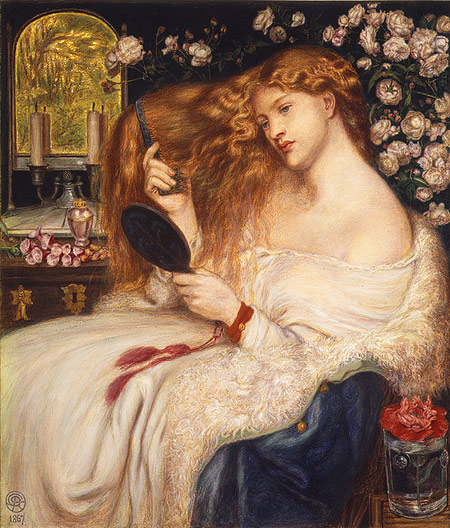
\includegraphics[width=0.40\textwidth]{Images/Rossetti_lady_lilith_1867}
	\\ {\small Rosetti 1867, Lady Lilith.}
\end{wrapfigure}


She, like Susan, was human once. She was the first woman. You see, women did not actually come from Adams rib. At least not the first. Lilith and Adam were both created from the dust to be each others companion. Adam preferred for her to be obedient to him and she preferred to have an equal partner and when that didn't work out she left. God only knows where she went but along the way she met Sam\ae l and they have been inseparable ever since.

She is the worlds first polyamorous woman. Sam\ae l may be her primary so to speak but she has had many lovers. Unlike the accusations of her being a whore though she genuinely loves those she is with and is quite happy, her and Sam\ae l are still together so they are an example of a successful polyamorous relationship.

She is a fierce advocate of women's sexuality, she enjoys sex with both men and women(not physically I assume, she's a d\ae mon), so as a result is an LGBT advocate. I'm sure that she is a 3rd generation feminist. She protects pregnant women and children. She is a healer. Although she heals through the feminine current she heals both men and women, especially with self image.

She is drop dead gorgeous. Everyone who sees her sees her differently but the description I was given makes her sound like an irish sex god. Long wavy red hair, pale skin and red lips, deep emerald green eyes, perfect body. She either wears nothing or majestic see through clothing.

What I have said I have said. There is such a conflicting mess in the field of demonology. Lilith likely has a dozen names at least. Her three most popular are Lilith, Lamia and Lamashtu. Sure they could be different entities but Lamashtu for one was described as being the daughter of heaven. In the context given it meant that God created her from nothing, as opposed to coming from man or woman. That has to be Lilith. 

Why is Lilith often described as evil incarnate? Sexually liberated feminist women and LGBT people are discriminated against now, whether they were Gods or not how would people have treated them or spoken of them in 1000BC or even before? People are so quick to see monsters around them, if only they would spend that time looking for the monsters inside themselves.
\end{comment}
\chapter{Legal Licence}
The media source is available at \textit{https://eteepell.github.io/Susans-Requiem} under the following license.\\

Creative Commons Attribution-ShareAlike 4.0 International Public License

By exercising the Licensed Rights (defined below), You accept and agree to be bound by the terms and conditions of this Creative Commons Attribution-ShareAlike 4.0 International Public License ("Public License"). To the extent this Public License may be interpreted as a contract, You are granted the Licensed Rights in consideration of Your acceptance of these terms and conditions, and the Licensor grants You such rights in consideration of benefits the Licensor receives from making the Licensed Material available under these terms and conditions.

Section 1 – Definitions.

    Adapted Material means material subject to Copyright and Similar Rights that is derived from or based upon the Licensed Material and in which the Licensed Material is translated, altered, arranged, transformed, or otherwise modified in a manner requiring permission under the Copyright and Similar Rights held by the Licensor. For purposes of this Public License, where the Licensed Material is a musical work, performance, or sound recording, Adapted Material is always produced where the Licensed Material is synched in timed relation with a moving image.
    Adapter's License means the license You apply to Your Copyright and Similar Rights in Your contributions to Adapted Material in accordance with the terms and conditions of this Public License.
    BY-SA Compatible License means a license listed at creativecommons.org/compatiblelicenses, approved by Creative Commons as essentially the equivalent of this Public License.
    Copyright and Similar Rights means copyright and/or similar rights closely related to copyright including, without limitation, performance, broadcast, sound recording, and Sui Generis Database Rights, without regard to how the rights are labeled or categorized. For purposes of this Public License, the rights specified in Section 2(b)(1)-(2) are not Copyright and Similar Rights.
    Effective Technological Measures means those measures that, in the absence of proper authority, may not be circumvented under laws fulfilling obligations under Article 11 of the WIPO Copyright Treaty adopted on December 20, 1996, and/or similar international agreements.
    Exceptions and Limitations means fair use, fair dealing, and/or any other exception or limitation to Copyright and Similar Rights that applies to Your use of the Licensed Material.
    License Elements means the license attributes listed in the name of a Creative Commons Public License. The License Elements of this Public License are Attribution and ShareAlike.
    Licensed Material means the artistic or literary work, database, or other material to which the Licensor applied this Public License.
    Licensed Rights means the rights granted to You subject to the terms and conditions of this Public License, which are limited to all Copyright and Similar Rights that apply to Your use of the Licensed Material and that the Licensor has authority to license.
    Licensor means the individual(s) or entity(ies) granting rights under this Public License.
    Share means to provide material to the public by any means or process that requires permission under the Licensed Rights, such as reproduction, public display, public performance, distribution, dissemination, communication, or importation, and to make material available to the public including in ways that members of the public may access the material from a place and at a time individually chosen by them.
    Sui Generis Database Rights means rights other than copyright resulting from Directive 96/9/EC of the European Parliament and of the Council of 11 March 1996 on the legal protection of databases, as amended and/or succeeded, as well as other essentially equivalent rights anywhere in the world.
    You means the individual or entity exercising the Licensed Rights under this Public License. Your has a corresponding meaning.

Section 2 – Scope.

    License grant.
        Subject to the terms and conditions of this Public License, the Licensor hereby grants You a worldwide, royalty-free, non-sublicensable, non-exclusive, irrevocable license to exercise the Licensed Rights in the Licensed Material to:
            reproduce and Share the Licensed Material, in whole or in part; and
            produce, reproduce, and Share Adapted Material.
        Exceptions and Limitations. For the avoidance of doubt, where Exceptions and Limitations apply to Your use, this Public License does not apply, and You do not need to comply with its terms and conditions.
        Term. The term of this Public License is specified in Section 6(a).
        Media and formats; technical modifications allowed. The Licensor authorizes You to exercise the Licensed Rights in all media and formats whether now known or hereafter created, and to make technical modifications necessary to do so. The Licensor waives and/or agrees not to assert any right or authority to forbid You from making technical modifications necessary to exercise the Licensed Rights, including technical modifications necessary to circumvent Effective Technological Measures. For purposes of this Public License, simply making modifications authorized by this Section 2(a)(4) never produces Adapted Material.
        Downstream recipients.
            Offer from the Licensor – Licensed Material. Every recipient of the Licensed Material automatically receives an offer from the Licensor to exercise the Licensed Rights under the terms and conditions of this Public License.
            Additional offer from the Licensor – Adapted Material. Every recipient of Adapted Material from You automatically receives an offer from the Licensor to exercise the Licensed Rights in the Adapted Material under the conditions of the Adapter’s License You apply.
            No downstream restrictions. You may not offer or impose any additional or different terms or conditions on, or apply any Effective Technological Measures to, the Licensed Material if doing so restricts exercise of the Licensed Rights by any recipient of the Licensed Material.
        No endorsement. Nothing in this Public License constitutes or may be construed as permission to assert or imply that You are, or that Your use of the Licensed Material is, connected with, or sponsored, endorsed, or granted official status by, the Licensor or others designated to receive attribution as provided in Section 3(a)(1)(A)(i).

    Other rights.
        Moral rights, such as the right of integrity, are not licensed under this Public License, nor are publicity, privacy, and/or other similar personality rights; however, to the extent possible, the Licensor waives and/or agrees not to assert any such rights held by the Licensor to the limited extent necessary to allow You to exercise the Licensed Rights, but not otherwise.
        Patent and trademark rights are not licensed under this Public License.
        To the extent possible, the Licensor waives any right to collect royalties from You for the exercise of the Licensed Rights, whether directly or through a collecting society under any voluntary or waivable statutory or compulsory licensing scheme. In all other cases the Licensor expressly reserves any right to collect such royalties.

Section 3 – License Conditions.

Your exercise of the Licensed Rights is expressly made subject to the following conditions.

    Attribution.

        If You Share the Licensed Material (including in modified form), You must:
            retain the following if it is supplied by the Licensor with the Licensed Material:
                identification of the creator(s) of the Licensed Material and any others designated to receive attribution, in any reasonable manner requested by the Licensor (including by pseudonym if designated);
                a copyright notice;
                a notice that refers to this Public License;
                a notice that refers to the disclaimer of warranties;
                a URI or hyperlink to the Licensed Material to the extent reasonably practicable;
            indicate if You modified the Licensed Material and retain an indication of any previous modifications; and
            indicate the Licensed Material is licensed under this Public License, and include the text of, or the URI or hyperlink to, this Public License.
        You may satisfy the conditions in Section 3(a)(1) in any reasonable manner based on the medium, means, and context in which You Share the Licensed Material. For example, it may be reasonable to satisfy the conditions by providing a URI or hyperlink to a resource that includes the required information.
        If requested by the Licensor, You must remove any of the information required by Section 3(a)(1)(A) to the extent reasonably practicable.
    ShareAlike.

    In addition to the conditions in Section 3(a), if You Share Adapted Material You produce, the following conditions also apply.
        The Adapter’s License You apply must be a Creative Commons license with the same License Elements, this version or later, or a BY-SA Compatible License.
        You must include the text of, or the URI or hyperlink to, the Adapter's License You apply. You may satisfy this condition in any reasonable manner based on the medium, means, and context in which You Share Adapted Material.
        You may not offer or impose any additional or different terms or conditions on, or apply any Effective Technological Measures to, Adapted Material that restrict exercise of the rights granted under the Adapter's License You apply.

Section 4 – Sui Generis Database Rights.

Where the Licensed Rights include Sui Generis Database Rights that apply to Your use of the Licensed Material:

    for the avoidance of doubt, Section 2(a)(1) grants You the right to extract, reuse, reproduce, and Share all or a substantial portion of the contents of the database;
    if You include all or a substantial portion of the database contents in a database in which You have Sui Generis Database Rights, then the database in which You have Sui Generis Database Rights (but not its individual contents) is Adapted Material, including for purposes of Section 3(b); and
    You must comply with the conditions in Section 3(a) if You Share all or a substantial portion of the contents of the database.

For the avoidance of doubt, this Section 4 supplements and does not replace Your obligations under this Public License where the Licensed Rights include other Copyright and Similar Rights.

Section 5 – Disclaimer of Warranties and Limitation of Liability.

    Unless otherwise separately undertaken by the Licensor, to the extent possible, the Licensor offers the Licensed Material as-is and as-available, and makes no representations or warranties of any kind concerning the Licensed Material, whether express, implied, statutory, or other. This includes, without limitation, warranties of title, merchantability, fitness for a particular purpose, non-infringement, absence of latent or other defects, accuracy, or the presence or absence of errors, whether or not known or discoverable. Where disclaimers of warranties are not allowed in full or in part, this disclaimer may not apply to You.
    To the extent possible, in no event will the Licensor be liable to You on any legal theory (including, without limitation, negligence) or otherwise for any direct, special, indirect, incidental, consequential, punitive, exemplary, or other losses, costs, expenses, or damages arising out of this Public License or use of the Licensed Material, even if the Licensor has been advised of the possibility of such losses, costs, expenses, or damages. Where a limitation of liability is not allowed in full or in part, this limitation may not apply to You.

    The disclaimer of warranties and limitation of liability provided above shall be interpreted in a manner that, to the extent possible, most closely approximates an absolute disclaimer and waiver of all liability.

Section 6 – Term and Termination.

    This Public License applies for the term of the Copyright and Similar Rights licensed here. However, if You fail to comply with this Public License, then Your rights under this Public License terminate automatically.

    Where Your right to use the Licensed Material has terminated under Section 6(a), it reinstates:
        automatically as of the date the violation is cured, provided it is cured within 30 days of Your discovery of the violation; or
        upon express reinstatement by the Licensor.
    For the avoidance of doubt, this Section 6(b) does not affect any right the Licensor may have to seek remedies for Your violations of this Public License.
    For the avoidance of doubt, the Licensor may also offer the Licensed Material under separate terms or conditions or stop distributing the Licensed Material at any time; however, doing so will not terminate this Public License.
    Sections 1, 5, 6, 7, and 8 survive termination of this Public License.

Section 7 – Other Terms and Conditions.

    The Licensor shall not be bound by any additional or different terms or conditions communicated by You unless expressly agreed.
    Any arrangements, understandings, or agreements regarding the Licensed Material not stated herein are separate from and independent of the terms and conditions of this Public License.

Section 8 – Interpretation.

    For the avoidance of doubt, this Public License does not, and shall not be interpreted to, reduce, limit, restrict, or impose conditions on any use of the Licensed Material that could lawfully be made without permission under this Public License.
    To the extent possible, if any provision of this Public License is deemed unenforceable, it shall be automatically reformed to the minimum extent necessary to make it enforceable. If the provision cannot be reformed, it shall be severed from this Public License without affecting the enforceability of the remaining terms and conditions.
    No term or condition of this Public License will be waived and no failure to comply consented to unless expressly agreed to by the Licensor.
    Nothing in this Public License constitutes or may be interpreted as a limitation upon, or waiver of, any privileges and immunities that apply to the Licensor or You, including from the legal processes of any jurisdiction or authority.

Creative Commons is not a party to its public licenses. Notwithstanding, Creative Commons may elect to apply one of its public licenses to material it publishes and in those instances will be considered the “Licensor.” The text of the Creative Commons public licenses is dedicated to the public domain under the CC0 Public Domain Dedication. Except for the limited purpose of indicating that material is shared under a Creative Commons public license or as otherwise permitted by the Creative Commons policies published at creativecommons.org/policies, Creative Commons does not authorize the use of the trademark “Creative Commons” or any other trademark or logo of Creative Commons without its prior written consent including, without limitation, in connection with any unauthorized modifications to any of its public licenses or any other arrangements, understandings, or agreements concerning use of licensed material. For the avoidance of doubt, this paragraph does not form part of the public licenses.

Creative Commons may be contacted at creativecommons.org.



% begin back matter

\end{document}
% END THE DOCUMENT


